
%Futuring Study material template- This template is designed for the soft copy
%This template is for the subject PHYSICS ONLY
%----------------------------------------------------------------------------------------
%	PACKAGES AND OTHER DOCUMENT CONFIGURATIONS
%----------------------------------------------------------------------------------------

\documentclass[11pt,fleqn,twoside]{book} % Default font size and left-justified equations

%%%
%----------------------------------------------------------------------------------------
%	VARIOUS REQUIRED PACKAGES AND CONFIGURATIONS
%----------------------------------------------------------------------------------------
\usepackage{eucal}
\usepackage{setspace}
\usepackage{bigints}
\usepackage{etoolbox}
\usepackage{dirtytalk}
\usepackage{epigraph}
\usepackage{physics}
\usepackage{amssymb}
\usepackage{chemfig}
\usepackage{stackrel}
\usepackage{scalerel}
\usepackage{longtable}
\usepackage{tabularx}
\usepackage{caption}
\usepackage{multirow}
\usepackage{environ}
\usepackage{subfigure}
\usepackage{graphicx} % Required for including pictures
\graphicspath{{Pictures/}{Pictures/sketching/}{Pictures/single and complex/}{Pictures/Coordinate system/}{Pictures/vector/}{Pictures/jamfigure/}{Pictures/conicsection/}{Pictures/conicsection/}{Pictures/electrostatics/}{Pictures/LCR/} {Pictures/BHU/}{Pictures/HCU/}{Pictures/Jest/}{Pictures/magnetostatics/}{Pictures/p-coulombs law/}{Pictures/p-vector/}{Pictures/quantum/}{Pictures/}{Pictures/BHU/}{Pictures/HCU/}{Pictures/JEST/} {Pictures/STR/}{Pictures/nuclear/} {Pictures/quantum/} {Pictures/Particle/} {Pictures/Newtons law/} {Pictures/work and energy/} {Pictures/Kinematics/}{Pictures/math prelim/} {Pictures/semiconductors/}{Pictures/Fluid mechanics/}{Pictures/Bipolar junction transistor/}{Pictures/Solid state/}{Pictures/digital/}{Pictures/Waves/}{Pictures/OPAMP/}{Pictures/Optics/}{Pictures/Wave Optics/}{Pictures/Net/}{Pictures/NET/}{Pictures/Gate/}{pictures/Newtons law/}{pictures/Kinematics/}{pictures/work and energy/}{pictures/jamfigure/}{Pictures/Problems/} {Pictures/Dirac delta function/}{Pictures/Differential equations/}{Pictures/Assignment/}{Pictures/Assignments/}
{Pictures/Electronics-CSIR/} {Pictures/CM/} {Pictures/Statistical Physics/}{Pictures/Digital Electronics/}{Pictures/Relativity and Electromagnetism/}{Pictures/Net 2019/}}
 % Specifies the directory where pictures are stored
\usepackage{float}
\usepackage{lipsum} % Inserts dummy text
\usepackage{wrapfig}
\usepackage{tikz} % Required for drawing custom shapes
\usepackage{amsmath}
 % English language/hyphenation

\usepackage{enumitem}
\newlist{questions}{enumerate}{3}
\setlist[questions]{wide=0pt, leftmargin=15pt, labelwidth=15pt, labelsep=0pt, align=left,label=\color{futuringtheme}\bfseries\large\arabic*.}
\newcommand{\question}{\item}


%\AtBeginEnvironment{enumerate}{\linespread{6.84}\selectfont}

 
 
\NewEnviron{abox}{%
	\begin{center}
\begin{tikzpicture}
\node[align=center,anchor=base,draw,rectangle,text width=\textwidth,line width=2pt,rounded corners=15pt,draw=ocre,fill=white,fill opacity=0.9,inner sep=10pt] 
{\centering \textbf{ \huge \color{futuringtheme}\BODY}};
\end{tikzpicture}

	\end{center}
	
	
}
\newcommand{\exyear}[1]{\newline \llap{}\hfill \color{futuringtheme}{\textbf{[#1]}}}
\usepackage{booktabs} % Required for nicer horizontal rules in tables
\usepackage{tasks}
\usepackage{xcolor} % Required for specifying colors by name
\definecolor{ocre}{RGB}{243,102,25} % Define the orange color used for highlighting throughout the book
\definecolor{futuringtheme}{RGB}{0,142,212}
%----------------------------------------------------------------------------------------
%..............................Added packages
\usepackage{import}
\usepackage{array}
\usepackage{colortbl}
\usepackage{cutwin}

\usepackage[printwatermark]{xwatermark}

\newsavebox\mylogobox
\savebox\mylogobox{\tikz[opacity=0.2]\node[inner sep=0pt] (russell) at (0,0)
	{
\includegraphics[width=3cm]{../Config/Pictures/logotra2.png}};}
\newwatermark*[
allpages,
angle=0,
scale=5,
xpos=0,
ypos=0
]{\usebox\mylogobox}



%.........................
%	MARGINS
%----------------------------------------------------------------------------------------
\usepackage{tasks}
\usepackage{geometry} % ccbyRequired for adjusting page dimensions and margins

\geometry{
	paper=a4paper, % Paper size, change to letterpaper for US letter size
	top=2cm, % Top margin
	bottom=2cm, % Bottom margin
	left=2cm, % Left margin
	right=2cm, % Right margin
	headheight=14pt, % Header height
	footskip=1.4cm, % Space from the bottom margin to the baseline of the footer
	headsep=10pt, % Space from the top margin to the baseline of the header
	%showframe, % Uncomment to show how the type block is set on the page
}

\allowdisplaybreaks
\makeatletter
\def\SetTotalwidth{\advance\linewidth by \@totalleftmargin
	\@totalleftmargin=0pt}
\makeatother

%----------------------------------------------------------------------------------------
%y

\usepackage{avant} % Use the Avantgarde font for headings
%\usepackage{times} % Use the Times font for headings
\usepackage{mathptmx} % Use the Adobe Times Roman as the default text font together with math symbols from the Sym­bol, Chancery and Com­puter Modern fonts

\usepackage{microtype} % Slightly tweak font spacing for aesthetics
\usepackage[utf8]{inputenc} % Required for including letters with accents
\usepackage[T1]{fontenc} % Use 8-bit encoding that has 256 glyphs

%----------------------------------------------------------------------------------------
%	BIBLIOGRAPHY AND INDEX
%----------------------------------------------------------------------------------------


%----------------------------------------------------------------------------------------
%	MAIN TABLE OF CONTENTS
%----------------------------------------------------------------------------------------

\usepackage{titletoc} % Required for manipulating the table of contents

\contentsmargin{0cm} % Removes the default margin

% Part text styling (this is mostly taken care of in the PART HEADINGS section of this file)
\titlecontents{part}
	[0cm] % Left indentation
	{\addvspace{20pt}\bfseries} % Spacing and font options for parts
	{}
	{}
	{}

% Chapter text styling
\titlecontents{chapter}
	[1.25cm] % Left indentation
	{\addvspace{12pt}\large\sffamily\bfseries} % Spacing and font options for chapters
	{\color{ocre!60}\contentslabel[\Large\thecontentslabel]{1.25cm}\color{ocre}} % Formatting of numbered sections of this type
	{\color{ocre}} % Formatting of numberless sections of this type
	{\color{ocre!60}\normalsize\;\titlerule*[.5pc]{.}\;\thecontentspage} % Formatting of the filler to the right of the heading and the page number

% Section text styling
\titlecontents{section}
	[1.25cm] % Left indentation
	{\addvspace{3pt}\sffamily\bfseries} % Spacing and font options for sections
	{\contentslabel[\thecontentslabel]{1.25cm}} % Formatting of numbered sections of this type
	{} % Formatting of numberless sections of this type
	{\hfill\color{black}\thecontentspage} % Formatting of the filler to the right of the heading and the page number

% Subsection text styling
\titlecontents{subsection}
	[1.25cm] % Left indentation
	{\addvspace{1pt}\sffamily\small} % Spacing and font options for subsections
	{\contentslabel[\thecontentslabel]{1.25cm}} % Formatting of numbered sections of this type
	{} % Formatting of numberless sections of this type
	{\ \titlerule*[.5pc]{.}\;\thecontentspage} % Formatting of the filler to the right of the heading and the page number

% Figure text styling
\titlecontents{figure}
	[1.25cm] % Left indentation
	{\addvspace{1pt}\sffamily\small} % Spacing and font options for figures
	{\thecontentslabel\hspace*{1em}} % Formatting of numbered sections of this type
	{} % Formatting of numberless sections of this type
	{\ \titlerule*[.5pc]{.}\;\thecontentspage} % Formatting of the filler to the right of the heading and the page number

% Table text styling
\titlecontents{table}
	[1.25cm] % Left indentation
	{\addvspace{1pt}\sffamily\small} % Spacing and font options for tables
	{\thecontentslabel\hspace*{1em}} % Formatting of numbered sections of this type
	{} % Formatting of numberless sections of this type
	{\ \titlerule*[.5pc]{.}\;\thecontentspage} % Formatting of the filler to the right of the heading and the page number

%----------------------------------------------------------------------------------------
%	MINI TABLE OF CONTENTS IN PART HEADS
%----------------------------------------------------------------------------------------

% Chapter text styling
\titlecontents{lchapter}
	[0em] % Left indentation
	{\addvspace{15pt}\large\sffamily\bfseries} % Spacing and font options for chapters
	{\color{ocre}\contentslabel[\Large\thecontentslabel]{1.25cm}\color{ocre}} % Chapter number
	{}  
	{\color{ocre}\normalsize\sffamily\bfseries\;\titlerule*[.5pc]{.}\;\thecontentspage} % Page number

% Section text styling
\titlecontents{lsection}
	[0em] % Left indentation
	{\sffamily\small} % Spacing and font options for sections
	{\contentslabel[\thecontentslabel]{1.25cm}} % Section number
	{}
	{}

% Subsection text styling (note these aren't shown by default, display them by searchings this file for tocdepth and reading the commented text)
\titlecontents{lsubsection}
	[.5em] % Left indentation
	{\sffamily\footnotesize} % Spacing and font options for subsections
	{\contentslabel[\thecontentslabel]{1.25cm}}
	{}
	{}

%----------------------------------------------------------------------------------------
%	HEADERS AND FOOTERS
%----------------------------------------------------------------------------------------

\usepackage{fancyhdr} % Required for header and footer configuration

\pagestyle{fancy} % Enable the custom headers and footers

\renewcommand{\chaptermark}[1]{\markboth{\sffamily\normalsize\bfseries\chaptername\ \thechapter.\ #1}{}} % Styling for the current chapter in the header
\renewcommand{\sectionmark}[1]{\markright{\sffamily\normalsize\thesection\hspace{5pt}#1}{}} % Styling for the current section in the header

\fancyhf{} % Clear default headers and footers
\fancyhead[LE,RO]{\sffamily\normalsize\thepage} % Styling for the page number in the header
\fancyhead[LO]{\rightmark} % Print the nearest section name on the left side of odd pages
\fancyhead[RE]{\leftmark} % Print the current chapter name on the right side of even pages
\renewcommand{\headrulewidth}{0.5pt} % Thickness of the rule under the header


% Removes the header from odd empty pages at the end of chapters
\makeatletter
\renewcommand{\cleardoublepage}{
\clearpage\ifodd\c@page\else
\hbox{}
\vspace*{\fill}
\thispagestyle{empty}
\newpage
\fi}


\fancypagestyle{plain}{% Redefine plain pages tyle
	\fancyhf{}% Clear header/footer
	
	\fancyhead[LE,RO]{\sffamily\normalsize\thepage}
	 % Print the nearest section name on the left side of odd pages
	\fancyhead[RE]{\leftmark}
}

%----------------------------------------------------------------------------------------

%Box Styles
\usepackage{tcolorbox}
\newtcolorbox{myboxthree}{colback=futuringtheme!5!white,colframe=ocre!75}






















%	THEOREM STYLES
%----------------------------------------------------------------------------------------

\usepackage{amsmath,amsfonts,amssymb,amsthm} % For math equations, theorems, symbols, etc

\newcommand{\intoo}[2]{\mathopen{]}#1\,;#2\mathclose{[}}
\newcommand{\ud}{\mathop{\mathrm{{}d}}\mathopen{}}
\newcommand{\intff}[2]{\mathopen{[}#1\,;#2\mathclose{]}}
\renewcommand{\qedsymbol}{$\blacksquare$}
\newtheorem{notation}{Notation}[chapter]

% Boxed/framed environments
\newtheoremstyle{ocrenumbox}% Theorem style name
{0pt}% Space above
{0pt}% Space below
{\normalfont}% Body font
{}% Indent amount
{\small\bf\sffamily\color{ocre}}% Theorem head font
{\;}% Punctuation after theorem head
{0.25em}% Space after theorem head
{\small\sffamily\color{ocre}\thmname{#1}\nobreakspace\thmnumber{\@ifnotempty{#1}{}\@upn{#2}}% Theorem text (e.g. Theorem 2.1)
\thmnote{\nobreakspace\the\thm@notefont\sffamily\bfseries\color{black}---\nobreakspace#3.}} % Optional theorem note

\newtheoremstyle{blacknumex}% Theorem style name
{5pt}% Space above
{5pt}% Space below
{\normalfont}% Body font
{} % Indent amount
{\small\bf\sffamily}% Theorem head font
{\;}% Punctuation after theorem head
{0.25em}% Space after theorem head
{\small\sffamily{\tiny\ensuremath{\blacksquare}}\nobreakspace\thmname{#1}\nobreakspace\thmnumber{\@ifnotempty{#1}{}\@upn{#2}}% Theorem text (e.g. Theorem 2.1)
\thmnote{\nobreakspace\the\thm@notefont\sffamily\bfseries---\nobreakspace#3.}}% Optional theorem note

\newtheoremstyle{blacknumbox} % Theorem style name
{0pt}% Space above
{0pt}% Space below
{\normalfont}% Body font
{}% Indent amount
{\small\bf\sffamily}% Theorem head font
{\;}% Punctuation after theorem head
{0.25em}% Space after theorem head
{\small\sffamily\thmname{#1}\nobreakspace\thmnumber{\@ifnotempty{#1}{}\@upn{#2}}% Theorem text (e.g. Theorem 2.1)
\thmnote{\nobreakspace\the\thm@notefont\sffamily\bfseries---\nobreakspace#3.}}% Optional theorem note

% Non-boxed/non-framed environments
\newtheoremstyle{ocrenum}% Theorem style name
{5pt}% Space above
{5pt}% Space below
{\normalfont}% Body font
{}% Indent amount
{\small\bf\sffamily\color{ocre}}% Theorem head font
{\;}% Punctuation after theorem head
{0.25em}% Space after theorem head
{\small\sffamily\color{ocre}\thmname{#1}\nobreakspace\thmnumber{\@ifnotempty{#1}{}\@upn{#2}}% Theorem text (e.g. Theorem 2.1)
\thmnote{\nobreakspace\the\thm@notefont\sffamily\bfseries\color{black}---\nobreakspace#3.}} % Optional theorem note
\makeatother

%Box style for Solution environment
\newtheoremstyle{solbox}% Theorem style name
{0pt}% Space above
{0pt}% Space below
{\normalfont}% Body font
{}% Indent amount
{\small\bf\sffamily\color{ocre}}% Theorem head font
{\;}% Punctuation after theorem head
{0.25em}% Space after theorem head
{\small\sffamily\color{ocre}Solution:}


% Defines the theorem text style for each type of theorem to one of the three styles above
\newcounter{dummy} 
\numberwithin{dummy}{section}
\theoremstyle{ocrenumbox}
\newtheorem{theoremeT}[dummy]{Theorem}
\newtheorem{problem}{Problem}[chapter]
\newtheorem{exerciseT}{Exercise}[chapter]
\theoremstyle{blacknumex}
\newtheorem{exampleT}{Example}[chapter]
\theoremstyle{blacknumbox}
\newtheorem{vocabulary}{Vocabulary}[chapter]
\newtheorem{definitionT}{Definition}[section]
\newtheorem{corollaryT}[dummy]{Corollary}
\theoremstyle{ocrenum}
\newtheorem{proposition}[dummy]{Proposition}
\theoremstyle{solbox}
\newtheorem{answerT}[dummy]{Solution}

%----------------------------------------------------------------------------------------
%	DEFINITION OF COLORED BOXES
%----------------------------------------------------------------------------------------

\RequirePackage[framemethod=default]{mdframed} % Required for creating the theorem, definition, exercise and corollary boxes

% Theorem box
\newmdenv[skipabove=7pt,
skipbelow=7pt,
backgroundcolor=white,
linecolor=ocre,
innerleftmargin=5pt,
innerrightmargin=5pt,
innertopmargin=10pt,
leftmargin=0cm,
rightmargin=0cm,
innerbottommargin=5pt]{tBox}

% Exercise box	  
\newmdenv[skipabove=7pt,
skipbelow=7pt,
rightline=false,
leftline=true,
topline=false,
bottomline=false,
backgroundcolor=ocre!10,
linecolor=ocre,
innerleftmargin=5pt,
innerrightmargin=5pt,
innertopmargin=5pt,
innerbottommargin=5pt,
leftmargin=0cm,
rightmargin=0cm,
linewidth=4pt]{eBox}	

% Definition box
\newmdenv[skipabove=7pt,
skipbelow=7pt,
rightline=false,
leftline=true,
topline=false,
bottomline=false,
linecolor=ocre,
innerleftmargin=5pt,
innerrightmargin=5pt,
innertopmargin=0pt,
leftmargin=0cm,
rightmargin=0cm,
linewidth=4pt,
innerbottommargin=0pt]{dBox}	

% Corollary box
\newmdenv[skipabove=7pt,
skipbelow=7pt,
rightline=false,
leftline=true,
topline=false,
bottomline=false,
linecolor=gray,
backgroundcolor=black!5,
innerleftmargin=5pt,
innerrightmargin=5pt,
innertopmargin=5pt,
leftmargin=0cm,
rightmargin=0cm,
linewidth=4pt,
innerbottommargin=5pt]{cBox}

% Creates an environment for each type of theorem and assigns it a theorem text style from the "Theorem Styles" section above and a colored box from above
\newenvironment{theorem}{\begin{tBox}\begin{theoremeT}}{\end{theoremeT}\end{tBox}}
\newenvironment{exercise}{\begin{eBox}\begin{exerciseT}}{\hfill{\color{ocre}\tiny\ensuremath{\blacksquare}}\end{exerciseT}\end{eBox}}				  
\newenvironment{definition}{\begin{dBox}\begin{definitionT}}{\end{definitionT}\end{dBox}}	
\newenvironment{example}{\begin{exampleT}}{\hfill{\tiny\ensuremath{\blacksquare}}\end{exampleT}}		
\newenvironment{corollary}{\begin{cBox}\begin{corollaryT}}{\end{corollaryT}\end{cBox}}	
\newenvironment{answer}{\begin{tBox}\begin{answerT}}{\end{answerT}\end{tBox}}	

%----------------------------------------------------------------------------------------
%	REMARK ENVIRONMENT
%----------------------------------------------------------------------------------------

\newenvironment{remark}{\par\vspace{10pt}\normlasize % Vertical white space above the remark and smaller font size
\begin{list}{}{
\leftmargin=35pt % Indentation on the left
\rightmargin=25pt}\item\ignorespaces % Indentation on the right
\makebox[-2.5pt]{\begin{tikzpicture}[overlay]
\node[draw=ocre!60,line width=1pt,circle,fill=ocre!25,font=\sffamily\bfseries,inner sep=2pt,outer sep=0pt] at (-15pt,0pt){\textcolor{ocre}{R}};\end{tikzpicture}} % Orange R in a circle
\advance\baselineskip -1pt}{\end{list}\vskip5pt} % Tighter line spacing and white space after remark

\newenvironment{note}{\par\vspace{10pt}\normalsize % Vertical white space above the remark and smaller font size
	\begin{list}{}{
			\leftmargin=35pt % Indentation on the left
			\rightmargin=25pt}\item\ignorespaces % Indentation on the right
		\makebox[-2.5pt]{\begin{tikzpicture}[overlay]
			\node[draw=ocre!60,line width=1pt,rectangle,fill=ocre!25,font=\sffamily\bfseries,inner sep=2pt,outer sep=0pt] at (-15pt,0pt){\textcolor{ocre}{Note}};\end{tikzpicture}} % Orange R in a circle
		\advance\baselineskip -5pt}{\end{list}\vskip5pt} % Tighter line spacing and white space after remark

%----------------------------------------------------------------------------------------
%	SECTION NUMBERING IN THE MARGIN
%----------------------------------------------------------------------------------------

\makeatletter
\renewcommand{\@seccntformat}[1]{\llap{\textcolor{ocre}{\csname the#1\endcsname}\hspace{1em}}}                    
\renewcommand{\section}{\@startsection{section}{1}{\z@}
{-4ex \@plus -1ex \@minus -.4ex}
{1ex \@plus.2ex }
{\normalfont\large\sffamily\bfseries}}
\renewcommand{\subsection}{\@startsection {subsection}{2}{\z@}
{-3ex \@plus -0.1ex \@minus -.4ex}
{0.5ex \@plus.2ex }
{\normalfont\sffamily\bfseries}}
\renewcommand{\subsubsection}{\@startsection {subsubsection}{3}{\z@}
{-2ex \@plus -0.1ex \@minus -.2ex}
{.2ex \@plus.2ex }
{\normalfont\small\sffamily\bfseries}}                        
\renewcommand\paragraph{\@startsection{paragraph}{4}{\z@}
{-2ex \@plus-.2ex \@minus .2ex}
{.1ex}
{\normalfont\small\sffamily\bfseries}}

%----------------------------------------------------------------------------------------
%	PART HEADINGS
%----------------------------------------------------------------------------------------

% Numbered part in the table of contents
\newcommand{\@mypartnumtocformat}[2]{%
	\setlength\fboxsep{0pt}%
	\noindent\colorbox{ocre!20}{\strut\parbox[c][.7cm]{\ecart}{\color{ocre!70}\Large\sffamily\bfseries\centering#1}}\hskip\esp\colorbox{ocre!40}{\strut\parbox[c][.7cm]{\linewidth-\ecart-\esp}{\Large\sffamily\centering#2}}%
}

% Unnumbered part in the table of contents
\newcommand{\@myparttocformat}[1]{%
	\setlength\fboxsep{0pt}%
	\noindent\colorbox{ocre!40}{\strut\parbox[c][.7cm]{\linewidth}{\Large\sffamily\centering#1}}%
}

\newlength\esp
\setlength\esp{4pt}
\newlength\ecart
\setlength\ecart{1.2cm-\esp}
\newcommand{\thepartimage}{}%
\newcommand{\partimage}[1]{\renewcommand{\thepartimage}{#1}}%
\def\@part[#1]#2{%
\ifnum \c@secnumdepth >-2\relax%
\refstepcounter{part}%
\addcontentsline{toc}{part}{\texorpdfstring{\protect\@mypartnumtocformat{\thepart}{#1}}{\partname~\thepart\ ---\ #1}}
\else%
\addcontentsline{toc}{part}{\texorpdfstring{\protect\@myparttocformat{#1}}{#1}}%
\fi%
\startcontents%
\markboth{}{}%
{\thispagestyle{empty}%
\begin{tikzpicture}[remember picture,overlay]%
\node at (current page.north west){\begin{tikzpicture}[remember picture,overlay]%	
\fill[ocre!20](0cm,0cm) rectangle (\paperwidth,-\paperheight);
\node[anchor=north] at (4cm,-3.25cm){\color{ocre!40}\fontsize{220}{100}\sffamily\bfseries\thepart}; 
\node[anchor=south east] at (\paperwidth-1cm,-\paperheight+1cm){\parbox[t][][t]{8.5cm}{
\printcontents{l}{0}{\setcounter{tocdepth}{1}}% The depth to which the Part mini table of contents displays headings; 0 for chapters only, 1 for chapters and sections and 2 for chapters, sections and subsections
}};
\node[anchor=north east] at (\paperwidth-1.5cm,-3.25cm){\parbox[t][][t]{15cm}{\strut\raggedleft\color{white}\fontsize{30}{30}\sffamily\bfseries#2}};
\end{tikzpicture}};
\end{tikzpicture}}%
\@endpart}
\def\@spart#1{%
\startcontents%
\phantomsection
{\thispagestyle{empty}%
\begin{tikzpicture}[remember picture,overlay]%
\node at (current page.north west){\begin{tikzpicture}[remember picture,overlay]%	
\fill[ocre!20](0cm,0cm) rectangle (\paperwidth,-\paperheight);
\node[anchor=north east] at (\paperwidth-1.5cm,-3.25cm){\parbox[t][][t]{15cm}{\strut\raggedleft\color{white}\fontsize{30}{30}\sffamily\bfseries#1}};
\end{tikzpicture}};
\end{tikzpicture}}
\addcontentsline{toc}{part}{\texorpdfstring{%
\setlength\fboxsep{0pt}%
\noindent\protect\colorbox{ocre!40}{\strut\protect\parbox[c][.7cm]{\linewidth}{\Large\sffamily\protect\centering #1\quad\mbox{}}}}{#1}}%
\@endpart}
\def\@endpart{\vfil\newpage
\if@twoside
\if@openright
\null
\thispagestyle{empty}%
\newpage
\fi
\fi
\if@tempswa
\twocolumn
\fi}

%----------------------------------------------------------------------------------------
%	CHAPTER HEADINGS
%----------------------------------------------------------------------------------------

% A switch to conditionally include a picture, implemented by Christian Hupfer
\newif\ifusechapterimage
\usechapterimagetrue
\newcommand{\thechapterimage}{}%
\newcommand{\chapterimage}[1]{\ifusechapterimage\renewcommand{\thechapterimage}{#1}\fi}%
\newcommand{\autodot}{.}
\def\@makechapterhead#1{%
{\parindent \z@ \raggedright \normalfont
\ifnum \c@secnumdepth >\m@ne
\if@mainmatter
\begin{tikzpicture}[remember picture,overlay]
\node at (current page.north west)
{\begin{tikzpicture}[remember picture,overlay]
\node[anchor=north west,inner sep=0pt] at (0,0) {\ifusechapterimage\includegraphics[width=\paperwidth]{\thechapterimage}\fi};
\draw[anchor=west] (\Gm@lmargin,-9cm) node [line width=2pt,rounded corners=15pt,draw=ocre,fill=white,fill opacity=0.5,inner sep=15pt]{\strut\makebox[22cm]{}};
\draw[anchor=west] (\Gm@lmargin+.3cm,-9cm) node {\huge\sffamily\bfseries\color{black}\thechapter\autodot~#1\strut};
\end{tikzpicture}};
\end{tikzpicture}
\else
\begin{tikzpicture}[remember picture,overlay]
\node at (current page.north west)
{\begin{tikzpicture}[remember picture,overlay]
\node[anchor=north west,inner sep=0pt] at (0,0) {\ifusechapterimage\includegraphics[width=\paperwidth]{\thechapterimage}\fi};
\draw[anchor=west] (\Gm@lmargin,-9cm) node [line width=2pt,rounded corners=15pt,draw=ocre,fill=white,fill opacity=0.5,inner sep=15pt]{\strut\makebox[22cm]{}};
\draw[anchor=west] (\Gm@lmargin+.3cm,-9cm) node {\huge\sffamily\bfseries\color{black}#1\strut};
\end{tikzpicture}};
\end{tikzpicture}
\fi\fi\par\vspace*{270\p@}}}

%-------------------------------------------

\def\@makeschapterhead#1{%
\begin{tikzpicture}[remember picture,overlay]
\node at (current page.north west)
{\begin{tikzpicture}[remember picture,overlay]
\node[anchor=north west,inner sep=0pt] at (0,0) {\ifusechapterimage\includegraphics[width=\paperwidth]{\thechapterimage}\fi};
\draw[anchor=west] (\Gm@lmargin,-9cm) node [line width=2pt,rounded corners=15pt,draw=ocre,fill=white,fill opacity=0.5,inner sep=15pt]{\strut\makebox[22cm]{}};
\draw[anchor=west] (\Gm@lmargin+.3cm,-9cm) node {\huge\sffamily\bfseries\color{black}#1\strut};
\end{tikzpicture}};
\end{tikzpicture}
\par\vspace*{270\p@}}
\makeatother

%----------------------------------------------------------------------------------------
%	LINKS
%----------------------------------------------------------------------------------------

\usepackage{hyperref}
\hypersetup{hidelinks,backref=true,pagebackref=true,hyperindex=true,colorlinks=false,breaklinks=true,urlcolor=ocre,bookmarks=true,bookmarksopen=false}

\usepackage{bookmark}
\bookmarksetup{
open,
numbered,
addtohook={%
\ifnum\bookmarkget{level}=0 % chapter
\bookmarksetup{bold}%
\fi
\ifnum\bookmarkget{level}=-1 % part
\bookmarksetup{color=ocre,bold}%
\fi
}
}
 % Insert the commands.tex file which contains the majority of the structure behind the template

\hypersetup{pdftitle={Title},pdfauthor={Futuring}} % Uncomment and fill out to include PDF metadata for the author and title of the book

%----------------------------------------------------------------------------------------

\begin{document}
\chapterimage{../../Config/Pictures/one.jpg}
%----------------------------------------------------------------------------------------
%	TITLE PAGE
%----------------------------------------------------------------------------------------

%Place the content from the snippet file titlepage and fill out the details -- Titlepage details
%----------------------------------------------------------------------------------------
%	COPYRIGHT PAGE
%----------------------------------------------------------------------------------------

%Place the content from the snippet file copyrightpage and fill out the details -- copyright details

%----------------------------------------------------------------------------------------
%	TABLE OF CONTENTS
%----------------------------------------------------------------------------------------



%----------------------------------------------------------------------------------------
%	CHAPTER 1
%----------------------------------------------------------------------------------------


\chapter{Power series Solution and Special functions}
\section{Series Solution Method}
Series expansion is a  method of obtaining one solution of the linear, second-order, homogeneous ODE. The method, will always work, provided the point of expansion is no worse than a regular singular point.In physics this very gentle condition is almost always satisfied. 
A linear, second-order, homogeneous ODE can be written in the form
\begin{equation}
\frac{d^{2} y}{d x^{2}}+P(x) \frac{d y}{d x}+Q(x) y=0 \label{DE002}
\end{equation}
The most general solution of the equation \ref{DE002} may be written as,
\begin{equation}
y(x)=c_{1} y_{1}(x)+c_{2} y_{2}(x)
\end{equation}
But a physical problem may lead to a nonhomogeneous, linear, second-order ODE
\begin{equation}
\frac{d^{2} y}{d x^{2}}+P(x) \frac{d y}{d x}+Q(x) y=F(x)\label{DE003}
\end{equation}
Hence the most general solution to the equation \label{DE003} will be of the form,
\begin{equation}
y(x)=c_{1} y_{1}(x)+c_{2} y_{2}(x)+y_{p}(x)
\end{equation}
The constants $c_{1}$ and $c_{2}$ will eventually be fixed by boundary conditions.\\\\
There are two series solution method  for differential equation,
\begin{enumerate}
	\item \textbf{Simple series expansion method}
	\item \textbf{Frobenious Method}
\end{enumerate}
\subsection{Simple Power Series Expansion Method}
The simple series expansion method works for differential equations whose solutions are well-behaved at the expansion point $x = 0$.
This method can be illustrated by Linear classical oscillator problem
\subsection{Classical Linear Oscillator}
\begin{align}
\frac{d^{2} y}{d x^{2}}+\omega^{2} y&=0 \label{DE003}\\
\text{with known solutions} \ y&=\sin \omega x, \cos \omega x\\
\text{We try}\ y(x) &=x^{k}\left(a_{0}+a_{1} x+a_{2} x^{2}+a_{3} x^{3}+\cdots\right) \\
&=\sum_{\lambda=0}^{\infty} a_{\lambda} x^{k+\lambda}, \quad a_{0} \neq 0 \label{DE004}\\
\intertext{with the exponent $k$ and all the coefficients $a_{\lambda}$ still undetermined. Note that $k$ need not be an integer. By differentiating twice, we obtain}
\frac{d y}{d x} &=\sum_{\lambda=0}^{\infty} a_{\lambda}(k+\lambda) x^{k+\lambda-1} \\
\frac{d^{2} y}{d x^{2}} &=\sum_{\lambda=0}^{\infty} a_{\lambda}(k+\lambda)(k+\lambda-1) x^{k+\lambda-2}
\intertext{By substituting into equation.\ref{DE003}, we have}
\sum_{\lambda=0}^{\infty} a_{\lambda}(k+\lambda)(k+\lambda-1) x^{k+\lambda-2}+\omega^{2} \sum_{\lambda=0}^{\infty} a_{\lambda} x^{k+\lambda}&=0 \label{DE005}
\intertext{The coefficients of each power of $x$ on the left-hand side of equation.\ref{DE005} must vanish individually.The lowest power of $x$ appearing in equation.\ref{DE005} is $x^{k-2}$, for $\lambda=0$ in the first summation. The requirement that the coefficient vanish  yields,}
a_{0} k(k-1)&=0
\intertext{We had chosen $a_{0}$ as the coefficient of the lowest nonvanishing terms of the series \ref{DE004}, hence, by definition, $a_{0} \neq 0$. Therefore we have,}
k(k-1)&=0 \label{DE006}
\end{align}
\textbf{This equation, coming from the coefficient of the lowest power of $x$, we call the {indicial equation}.} The indicial equation and its roots are of critical importance to our analysis.
\\From equation.\ref{DE006}, \qquad $k=0 $ or $k=1$\\
The only way a power series can be zero is, it's coefficients must be equal to zero. But here the power of $x$ in the equation do not match up. The Coefficent of $x$ in the first term is,${k+\lambda-2} $ and for the second term it is,$k+\lambda$, to make them equal, we can replace $\lambda$ by $\lambda+2$ in the first term. Then we get,
\begin{align}
\sum_{\lambda=2}^{\infty} a_{\lambda+2}(k+\lambda+2)(k+\lambda+1) x^{k+\lambda}+\omega^{2} \sum_{\lambda=0}^{\infty} a_{\lambda} x^{k+\lambda}&=0\\
\sum_{\lambda=2}^{\infty} a_{\lambda+2}(k+\lambda+2)(k+\lambda+1) +\omega^{2} \sum_{\lambda=0}^{\infty} a_{\lambda} &=0
\intertext{Here the coefficients  are independent summations and $\lambda $ is a dummy index. Then we get,}
a_{\lambda+2}(k+\lambda+2)(k+\lambda+1) +\omega^{2} a_{\lambda} &=0\\
a_{\lambda+2}&=-a_{\lambda} \frac{\omega^{2}}{(k+\lambda+2)(k+\lambda+1)}\label{DE007}
\end{align}
For this example, if we start with $a_{0}$, Equation.\ref{DE007} leads to the even coefficients $a_{2}, a_{4}$, and so on, and ignores $a_{1}, a_{3}, a_{5}$, and so on. Since $a_{1}$ is arbitrary if $k=0$ and necessarily zero if $k=1$, 
$$
a_{3}=a_{5}=a_{7}=\cdots=0
$$
and all the odd-numbered coefficients vanish. The odd powers of $x$ will actually reappear when the second root of the indicial equation is used.
\begin{align}
a_{\lambda+2}&=-a_{\lambda} \frac{\omega^{2}}{(\lambda+2)(\lambda+1)}
\intertext{which leads to}
a_{2}&=-a_{0} \frac{\omega^{2}}{1 \cdot 2}=-\frac{\omega^{2}}{2 !} a_{0} \\
a_{4}&=-a_{2} \frac{\omega^{2}}{3 \cdot 4}=+\frac{\omega^{4}}{4 !} a_{0} \\
a_{6}&=-a_{4} \frac{\omega^{2}}{5 \cdot 6}=-\frac{\omega^{6}}{6 !} a_{0}, \quad \text { and so on. }
\intertext{By inspection (and mathematical induction),}
a_{2 n}&=(-1)^{n} \frac{\omega^{2 n}}{(2 n) !} a_{0}
\intertext{and our solution is}
y(x)_{k=0}&=a_{0}\left[1-\frac{(\omega x)^{2}}{2 !}+\frac{(\omega x)^{4}}{4 !}-\frac{(\omega x)^{6}}{6 !}+\cdots\right]\\&=a_{0} \cos \omega x\\
\intertext{If we choose the indicial equation root $k=1$ Equation.\ref{DE007}, the recurrence relation becomes}
a_{j+2}&=-a_{j} \frac{\omega^{2}}{(j+3)(j+2)}\\
\intertext{Substituting in $j=0,2,4$, successively, we obtain}
a_{2}=-a_{0} \frac{\omega^{2}}{2 \cdot 3}&=-\frac{\omega^{2}}{3 !} a_{0} \\
a_{4}=-a_{2} \frac{\omega^{2}}{4 \cdot 5}&=+\frac{\omega^{4}}{5 !} a_{0} \\
a_{6}=-a_{4} \frac{\omega^{2}}{6 \cdot 7}&=-\frac{\omega^{6}}{7 !} a_{0}, \quad \text { and so on. }
\intertext{Again, by inspection and mathematical induction,}
a_{2 n}&=(-1)^{n} \frac{\omega^{2 n}}{(2 n+1) !} a_{0}\\
\intertext{For this choice, $k=1$, we obtain}
y(x)_{k=1} &=a_{0} x\left[1-\frac{(\omega x)^{2}}{3 !}+\frac{(\omega x)^{4}}{5 !}-\frac{(\omega x)^{6}}{7 !}+\cdots\right] \\
&=\frac{a_{0}}{\omega}\left[(\omega x)-\frac{(\omega x)^{3}}{3 !}+\frac{(\omega x)^{5}}{5 !}-\frac{(\omega x)^{7}}{7 !}+\cdots\right] \\
&=\frac{a_{0}}{\omega} \sin \omega x
\end{align}
\subsubsection{Power Series Solution (About an Ordinary Point)}
Find the power series solution of $\left(1-x^{2}\right) y^{\prime \prime}-2 x y^{\prime}+2 y=0$ about $x=0$\\\\
Since $x=0$ is an ordinary point of the given differential equation, the solution can be written as
\begin{align*}
y&=\sum_{k=0}^{\infty} a_{k} x^{k} \\ \frac{d y}{d x}&=\sum_{k=0}^{\infty} k a_{k} x^{k-1} \\ \frac{d^{2} y}{d x^{2}}&=\sum_{k=0}^{\infty} a_{k} k(k-1) x^{k-2}
\intertext{Substituting these values in the given equation we get,}
\left(1-x^{2}\right) \sum_{k} a_{k} k(k-1) x^{k-2}&-2 x \sum_{k} a_{k}(k) x^{k-1}+2 \sum_{k} a_{k} x^{k}=0 \\
\sum_{k=2} a_{k} k(k-1) x^{k-2}&-\sum\left(k^{2}+k-2\right) a_{k} x^{k}=0
\intertext{now equating the coefficient of $x^{k}$ then}
(k+2)(k+1) a_{k+2}-\left(k^{2}+k-2\right) a_{k}&=0 \\a_{k+2}&=\frac{k-1}{(k+1)} a_{k}\\
\text{For} \ k&=0 \Rightarrow a_{2}=-a_{0} \\ k&=1 \Rightarrow a_{3}=0 \\
k&=2 \Rightarrow a_{4}=\frac{a_{2}}{3}=\frac{-a_{0}}{3}  \\ k&=3 \Rightarrow a_{5}=\frac{2}{4} a_{3}=0\\
\text{Therefore, solution}\ y&=a_{0}+a_{1} x+a_{2} x^{2}+\ldots \ldots\\&=a_{0}\left[1-x^{2}-\frac{x^{4}}{3} \ldots . .\right]+a_{1} x
\end{align*}
\subsection{Frobenious Method}
Even though the simple power series expansion method works for many functions there are some whose behaviour  precludes the simple series method like the Bessel's function. The need of Frobenious method  lies under the fact that, \textbf{any functions involving negative or fractional powers would not be amenable to power series solution method}. The Frobenious method extends the simple power series solution method to include negative and fractional powers, and it also allows a natural extension involving logarithm terms.\\
The basic idea of the Frobenius method is to look for solutions of the form
\begin{align*}
y(x) &=a_{0} x^{\lambda}+a_{1} x^{\lambda+1}+a_{2} x^{\lambda+2}+a_{3} x^{\lambda+3}+\ldots \\
&=x^{\lambda}\left(a_{0}+a_{1} x+a_{2} x^{2}+a_{3} x^{3}+\ldots\right) \\
&=x^{\lambda} \sum_{k=0}^{\infty} a_{k} x^{k} \\
&= \sum_{k=0}^{\infty} a_{k} x^{k+\lambda}
\end{align*}
The extension of the simple power series method is all in the factor $x^{\lambda}$. The power $c$ must now be determined, as well as the coefficients $a_{k}$. Since $\lambda$ may be negative, positive, and possibly non-integral, this extends considerably the range of functions which may be treated. Note that $a_{0}$ is the lowest non-zero coefficient, so by definition it cannot be zero.
\subsection{Bessel Function}
\newpage
\begin{abox}
	Problem Set -1
\end{abox}
\begin{enumerate}[label=\color{ocre}\textbf{\arabic*.}]
	\item  Let $p_{n}(x)$ (where $n=0,1,2, \ldots \ldots$ ) be a polynomial of degree $n$ with real coefficients, defined in the interval $2 \leq n \leq 4$. If $\int_{2}^{4} p_{n}(x) p_{m}(x) d x=\delta_{n m}$, then
	{\exyear{NET/JRF(JUNE-2011)}}
	\begin{tasks}(2)
		\task[\textbf{A.}] $p_{0}(x)=\frac{1}{\sqrt{2}}$ and $p_{1}(x)=\sqrt{\frac{3}{2}}(-3-x)$
		\task[\textbf{B.}]  $p_{0}(x)=\frac{1}{\sqrt{2}}$ and $p_{1}(x)=\sqrt{3}(3+x)$
		\task[\textbf{C.}] $p_{0}(x)=\frac{1}{2}$ and $p_{1}(x)=\sqrt{\frac{3}{2}}(3-x)$
		\task[\textbf{D.}] $p_{0}(x)=\frac{1}{\sqrt{2}}$ and $p_{1}(x)=\sqrt{\frac{3}{2}}(3-x)$
	\end{tasks}
	\item  The generating function $F(x, t)=\sum_{n=0}^{\infty} P_{n}(x) t^{n}$ for the Legendre polynomials $P_{n}(x)$ is $F(x, t)=\left(1-2 x t+t^{2}\right)^{-1 / 2}$. The value of $P_{3}(-1)$ is
	{\exyear{NET/JRF(DEC-2011)}}
	\begin{tasks}(4)
		\task[\textbf{A.}] $5 / 2$
		\task[\textbf{B.}] $3 / 2$
		\task[\textbf{C.}] $+1$
		\task[\textbf{D.}] $-1$
	\end{tasks}
	\item  The graph of the function $f(x)$ shown below is best described by
	{\exyear{NET/JRF(DEC-2012)}}
	\begin{figure}[H]
		\centering
		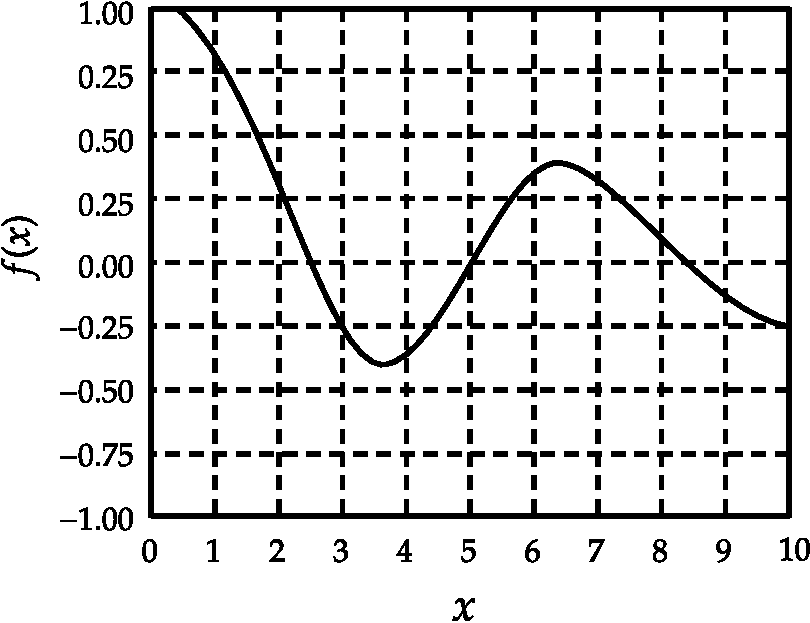
\includegraphics[height=6cm,width=8cm]{diagram-20211005(12)-crop}
	\end{figure}
	\begin{tasks}(2)
		\task[\textbf{A.}]  The Bessel function $J_{0}(x)$
		\task[\textbf{B.}] $\cos x$
		\task[\textbf{C.}] $e^{-x} \cos x$
		\task[\textbf{D.}] $\frac{1}{x} \cos x$
	\end{tasks}
	\item Given that $\sum_{n=0}^{\infty} H_{n}(x) \frac{t^{n}}{n !}=e^{-t^{2}+2 t x}$ the value of $H_{4}(0)$ is
	{\exyear{NET/JRF(JUNE-2013)}}
	\begin{tasks}(4)
		\task[\textbf{A.}] 12
		\task[\textbf{B.}] 6
		\task[\textbf{C.}] 24
		\task[\textbf{D.}] $-6$
	\end{tasks}
	\item   Given $\sum_{n=0}^{\infty} P_{n}(x) t^{n}=\left(1-2 x t+t^{2}\right)^{-1 / 2}$, for $|t|<1$, the value of $P_{5}(-1)$ is
	{\exyear{NET/JRF(JUNE-2014)}}
	\begin{tasks}(4)
		\task[\textbf{A.}] $0.26$
		\task[\textbf{B.}] 1
		\task[\textbf{C.}] $0.5$
		\task[\textbf{D.}] $-1$
	\end{tasks}
	\item The function $f(x)=\sum_{n=0}^{\infty} \frac{(-1)^{n}}{n !(n+1) !}\left(\frac{x}{2}\right)^{2 n+1}$, satisfies the differential equation
	{\exyear{NET/JRF(DEC-2014)}}
	\begin{tasks}(2)
		\task[\textbf{A.}]  $x^{2} \frac{d^{2} f}{d x^{2}}+x \frac{d f}{d x}+\left(x^{2}+1\right) f=0$
		\task[\textbf{B.}]  $x^{2} \frac{d^{2} f}{d x^{2}}+2 x \frac{d f}{d x}+\left(x^{2}-1\right) f=0$
		\task[\textbf{C.}] $x^{2} \frac{d^{2} f}{d x^{2}}+x \frac{d f}{d x}+\left(x^{2}-1\right) f=0$
		\task[\textbf{D.}] $x^{2} \frac{d^{2} f}{d x^{2}}-x \frac{d f}{d x}+\left(x^{2}-1\right) f=0$
	\end{tasks}
	\item
	 The Hermite polynomial $H_{n}(x)$, satisfies the differential equation
	$$
	\frac{d^{2} H_{n}}{d x^{2}}-2 x \frac{d H_{n}}{d x}+2 n H_{n}(x)=0
	$$
	The corresponding generating function $G(t, x)=\sum_{n=0}^{\infty} \frac{1}{n !} H_{n}(x) t^{n}$, satisfies the equation
	{\exyear{NET/JRF(DEC-2015)}}
	\begin{tasks}(2)
		\task[\textbf{A.}] $\frac{\partial^{2} G}{\partial x^{2}}-2 x \frac{\partial G}{\partial x}+2 t \frac{\partial G}{\partial t}=0$
		\task[\textbf{B.}] $\frac{\partial^{2} G}{\partial x^{2}}-2 x \frac{\partial G}{\partial x}-2 t^{2} \frac{\partial G}{\partial t}=0$
		\task[\textbf{C.}] $\frac{\partial^{2} G}{\partial x^{2}}-2 x \frac{\partial G}{\partial x}+2 \frac{\partial G}{\partial t}=0$
		\task[\textbf{D.}]  $\frac{\partial^{2} G}{\partial x^{2}}-2 x \frac{\partial G}{\partial x}+2 \frac{\partial^{2} G}{\partial x \partial t}=0$
	\end{tasks}
	\item A stable asymptotic solution of the equation $x_{n+1}=1+\frac{3}{1+x_{n}}$ is $x=2$. If we take $x_{n}=2+\epsilon_{n}$ and $x_{n+1}=2+\epsilon_{n+1}$, where $\epsilon_{n}$ and $\epsilon_{n+1}$ are both small, the ratio $\frac{\epsilon_{n+1}}{\epsilon_{n}}$ is approximately
	{\exyear{NET/JRF(DEC-2016)}}
	\begin{tasks}(4)
		\task[\textbf{A.}] $-\frac{1}{2}$
		\task[\textbf{B.}] $-\frac{1}{4}$
		\task[\textbf{C.}]  $-\frac{1}{3}$
		\task[\textbf{D.}] $-\frac{2}{3}$
	\end{tasks}
	\item  The Green's function satisfying
	$$
	\frac{d^{2}}{d x^{2}} g\left(x, x_{0}\right)=\delta\left(x-x_{0}\right)
	$$
	with the boundary conditions $g\left(-L, x_{0}\right)=0=g\left(L, x_{0}\right)$, is
	{\exyear{NET/JRF(JUNE-2017)}}
	\begin{tasks}(1)
		\task[\textbf{A.}] $\left\{\begin{array}{ll}\frac{1}{2 L}\left(x_{0}-L\right)(x+L), & -L \leq x<x_{0} \\ \frac{1}{2 L}\left(x_{0}+L\right)(x-L), & x_{0} \leq x \leq L\end{array}\right.$
		\task[\textbf{B.}]  $\left\{\begin{array}{ll}\frac{1}{2 L}\left(x_{0}+L\right)(x+L), & -L \leq x<x_{0} \\ \frac{1}{2 L}\left(x_{0}-L\right)(x-L), & x_{0} \leq x \leq L\end{array}\right.$
		\task[\textbf{C.}] $\left\{\begin{array}{ll}\frac{1}{2 L}\left(L-x_{0}\right)(x+L), & -L \leq x<x_{0} \\ \frac{1}{2 L}\left(x_{0}+L\right)(L-x), & x_{0} \leq x \leq L\end{array}\right.$
		\task[\textbf{D.}] $\frac{1}{2 L}(x-L)(x+L), \quad-L \leq x \leq L$
	\end{tasks}
	\item  The generating function $G(t, x)$ for the Legendre polynomials $P_{n}(t)$ is
	$$
	G(t, x)=\frac{1}{\sqrt{1-2 x t+x^{2}}}=\sum_{n=0}^{\infty} x^{n} P_{n}(t), \text { for }|x|<1
	$$
	If the function $f(x)$ is defined by the integral equation $\int_{0}^{x} f\left(x^{\prime}\right) d x^{\prime}=x G(1, x)$, it can be expressed as
	{\exyear{NET/JRF(DEC-2017)}}
	\begin{tasks}(2)
		\task[\textbf{A.}] $\sum_{n, m=0}^{\infty} x^{n+m} P_{n}(1) P_{m}\left(\frac{1}{2}\right)$
		\task[\textbf{B.}] $\sum_{n, m=0}^{\infty} x^{n+m} P_{n}(1) P_{m}(1)$
		\task[\textbf{C.}] $\sum_{n, m=0}^{\infty} x^{n-m} P_{n}(1) P_{m}(1)$
		\task[\textbf{D.}] $\sum_{n, m=0}^{\infty} x^{n-m} P_{n}(0) P_{m}(1)$
	\end{tasks}
	\item In the function $P_{n}(x) e^{-x^{2}}$ of a real variable $x, P_{n}(x)$ is polynomial of degree $n$. The maximum number of extrema that this function can have is
	{\exyear{NET/JRF(JUNE-2018)}}
	\begin{tasks}(4)
		\task[\textbf{A.}] $n+2$
		\task[\textbf{B.}]  $n-1$
		\task[\textbf{C.}] $n+1$
		\task[\textbf{D.}] $n$
	\end{tasks}
	\item  The Green's function $G\left(x, x^{\prime}\right)$ for the equation $\frac{d^{2} y(x)}{d x^{2}}+y(x)=f(x)$, with the boundary values $y(0)=y\left(\frac{\pi}{2}\right)=0$, is
	{\exyear{NET/JRF(JUNE-2018)}}
	\begin{tasks}(1)
		\task[\textbf{A.}] $G\left(x, x^{\prime}\right)=\left\{\begin{array}{ll}x\left(x^{\prime}-\frac{\pi}{2}\right), & 0<x<x^{\prime}<\frac{\pi}{2} \\ \left(x-\frac{\pi}{2}\right) x^{\prime}, & 0<x^{\prime}<x<\frac{\pi}{2}\end{array}\right.$
		\task[\textbf{B.}] $G\left(x, x^{\prime}\right)=\left\{\begin{array}{ll}-\cos x^{\prime} \sin x, & 0<x<x^{\prime}<\frac{\pi}{2} \\ -\sin x^{\prime} \cos x, & 0<x^{\prime}<x<\frac{\pi}{2}\end{array}\right.$
		\task[\textbf{C.}] $G\left(x, x^{\prime}\right)=\left\{\begin{array}{ll}\cos x^{\prime} \sin x, & 0<x<x^{\prime}<\frac{\pi}{2} \\ \sin x^{\prime} \cos x, & 0<x^{\prime}<x<\frac{\pi}{2}\end{array}\right.$
		\task[\textbf{D.}] $G\left(x, x^{\prime}\right)=\left\{\begin{array}{ll}x\left(\frac{\pi}{2}-x^{\prime}\right), & 0<x<x^{\prime}<\frac{\pi}{2} \\ x^{\prime}\left(\frac{\pi}{2}-x\right), & 0<x^{\prime}<x<\frac{\pi}{2}\end{array}\right.$
	\end{tasks}
	\item The polynomial $f(x)=1+5 x+3 x^{2}$ is written as linear combination of the Legendre polynomials
	$\left(P_{0}(x)=1, P_{1}(x), P_{2}(x)=\frac{1}{2}\left(3 x^{2}-1\right)\right)$ as $f(x)=\sum_{n} c_{n} P_{n}(x)$. The value of $c_{0}$ is
	{\exyear{NET/JRF(DEC-2018)}}
	\begin{tasks}(4)
		\task[\textbf{A.}] $\frac{1}{4}$
		\task[\textbf{B.}] $\frac{1}{2}$
		\task[\textbf{C.}]  2
		\task[\textbf{D.}]  4
	\end{tasks}
	\item The Green's function $G\left(x, x^{\prime}\right)$ for the equation $\frac{d^{2} y(x)}{d x^{2}}=f(x)$, with the boundary values $y(0)=0$ and $y(1)=0$, is
	{\exyear{NET/JRF(DEC-2018)}}
	\begin{tasks}(1)
		\task[\textbf{A.}] $G\left(x, x^{\prime}\right)=\left\{\begin{array}{ll}\frac{1}{2} x\left(1-x^{\prime}\right), & 0<x<x^{\prime}<1 \\ \frac{1}{2} x^{\prime}(1-x) & 0<x^{\prime}<x<1\end{array}\right.$
		\task[\textbf{B.}] $G\left(x, x^{\prime}\right)=\left\{\begin{array}{ll}x\left(x^{\prime}-1\right), & 0<x<x^{\prime}<1 \\ x^{\prime}(1-x) & 0<x^{\prime}<x<1\end{array}\right.$
		\task[\textbf{C.}] $G\left(x, x^{\prime}\right)=\left\{\begin{array}{ll}-\frac{1}{2} x\left(1-x^{\prime}\right), & 0<x<x^{\prime}<1 \\ \frac{1}{2} x^{\prime}(1-x) & 0<x^{\prime}<x<1\end{array}\right.$
		\task[\textbf{D.}]  $G\left(x, x^{\prime}\right)=\left\{\begin{array}{ll}x\left(x^{\prime}-1\right), & 0<x<x^{\prime}<1 \\ x^{\prime}(x-1) & 0<x^{\prime}<x<1\end{array}\right.$
	\end{tasks}
	\item  The Green's function for the differential equation $\frac{d^{2} x}{d t^{2}}+x=f(t)$, satisfying the initial conditions $x(0)=\frac{d x}{d t}(0)=0$ is\\
	$$G(t, \tau)=\left\{\begin{array}{ll}0 & \text { for } \quad 0<t<\tau \\ \sin (t-\tau) & \text { for } \quad t>\tau\end{array}\right.$$\\
	The solution of the differential equation when the source $f(t)=\theta(t)$ (the Heaviside step function) is
	{\exyear{NET/JRF(JUNE-2020)}}
	\begin{tasks}(4)
		\task[\textbf{A.}] $\sin t$
		\task[\textbf{B.}] $1-\sin t$
		\task[\textbf{C.}] $1-\cos t$
		\task[\textbf{D.}] $\cos ^{2} t-1$
	\end{tasks}
\end{enumerate}
 \colorlet{ocre1}{ocre!70!}
\colorlet{ocrel}{ocre!30!}
\setlength\arrayrulewidth{1pt}
\begin{table}[H]
	\centering
	\arrayrulecolor{ocre}
	\begin{tabular}{|p{1.5cm}|p{1.5cm}||p{1.5cm}|p{1.5cm}|}
		\hline
		\multicolumn{4}{|c|}{\textbf{Answer key}}\\\hline\hline
		\rowcolor{ocrel}Q.No.&Answer&Q.No.&Answer\\\hline
		1&\textbf{D} &2&\textbf{D}\\\hline 
		3&\textbf{A} &4&\textbf{A} \\\hline
		5&\textbf{D} &6&\textbf{C} \\\hline
		7&\textbf{A}&8&\textbf{C}\\\hline
		9&\textbf{A}&10&\textbf{B}\\\hline
		11&\textbf{C} &12&\textbf{B}\\\hline
		13&\textbf{C}&14&\textbf{D}\\\hline
		15&\textbf{C}& &\\\hline
		
	\end{tabular}
\end{table}
\begin{abox}
	Problem Set -3
\end{abox}
\begin{enumerate}[label=\color{ocre}\textbf{\arabic*.}]
	\item Green function for time dependent Schrödinger wave equation is defined as $G\left(\vec{r}, t: r^{\prime}, t^{\prime}\right)$. If $H$ is Hamiltonion of system then $G\left(\vec{r}, t: r^{\prime}, t^{\prime}\right)$ will satisfied the equation
	 \begin{tasks}(1)
		\task[\textbf{a.}]$\left(i \hbar \frac{\partial}{\partial t}-H\right) G\left(\vec{r}, t ; \vec{r}^{\prime}, t^{\prime}\right)=0$
		\task[\textbf{b.}]$\left(i \hbar \frac{\partial}{\partial t}-H\right) G\left(\vec{r}, t ; \vec{r}^{\prime}, t^{\prime}\right)=\delta\left(\vec{r}-\vec{r}^{\prime}\right)$
		\task[\textbf{c.}] $\left(i \hbar \frac{\partial}{\partial t}-H\right) G\left(\vec{r}, t ; \vec{r}^{\prime}, t^{\prime}\right)=\delta\left(t-t^{\prime}\right)$
		\task[\textbf{d.}]  $\left(i \hbar \frac{\partial}{\partial t}-H\right) G\left(\vec{r}, t ; \vec{r}^{\prime}, t^{\prime}\right)=\delta\left(\vec{r}-\vec{r}^{\prime}\right) \delta\left(t-t^{\prime}\right)$
	\end{tasks}
\begin{answer}
So the correct answer is \textbf{Option (d)}
\end{answer}
	\item $G\left(x, x_{0}\right)$ is the Green's function associated with the boundary value problem consisting of ordinary differential equation.
	$$
	\frac{d}{d x}\left(p(x) \frac{d u}{d x}\right)=f(x) \text { with } u(0)=0, u(L)=0
	$$
	The discontinuity condition on the derivative $\frac{d G\left(x, x_{0}\right)}{d x}$ at $x=x_{0}$ is
	 \begin{tasks}(4)
		\task[\textbf{a.}]0
		\task[\textbf{b.}]$p\left(x_{0}\right)$
		\task[\textbf{c.}]1
		\task[\textbf{d.}] $\frac{1}{p\left(x_{0}\right)}$
	\end{tasks}
\begin{answer}
	\begin{align*}
	\left.\frac{d G}{d x}\right|_{x=x_{0}^{+}}-\left.\frac{d G}{d x}\right|_{x=x_{i 1}^{-}}=\frac{1}{p\left(x_{0}\right)}
	\end{align*}
	So the correct answer is \textbf{Option (d)}
\end{answer}
\item Consider the steady state heat equation $\frac{d^{2} u}{d x^{2}}=f(x)$ with boundary condition,
$$
u(0)=0, u(L)=0
$$
The Green's function associated with the above equation
 \begin{tasks}(2)
	\task[\textbf{a.}]Constant
	\task[\textbf{b.}] Linear function
	\task[\textbf{c.}] Parabolic function
	\task[\textbf{d.}] Hyperbolic function
\end{tasks}
\begin{answer}
	\begin{align*}
	\intertext{The Green's function satisfies}
	\frac{d^{2} G\left(x, x_{0}\right)}{d x^{2}}&=\delta\left(x-x_{0}\right)\\
\text{	with }G\left(0, x_{0}\right)&=0\text{ and }G\left(L, x_{0}\right)=0
\intertext{Corresponding homogeneous equation is:}
\frac{d^{2} G}{d x^{2}}&=0\\
\text{Solution for }x \neq x_{0}&\text{ are, }G\left(x, x_{0}\right)= \begin{cases}a+b x_{2} & x<x_{1+} \\ c+d x, & x>x_{0}\end{cases}
	\end{align*}
		So the correct answer is \textbf{Option (b)}
\end{answer}
\item Consider the steady state heat equation $\frac{d^{2} u}{d x^{2}}=f(x)$ with boundary condition. $u(0)=0, u(L)=0$
The Green's function associated with the above equation is
 \begin{tasks}(1)
	\task[\textbf{a.}] $G\left(x, x_{0}\right)= \begin{cases}\frac{x}{L}\left(x_{0}-L\right), & 0 \leq x \leq x_{0} \\ \frac{x_{0}}{L}(x-L), & x_{0} \leq x \leq L\end{cases}$
	\task[\textbf{b.}] $G\left(x, x_{0}\right)= \begin{cases}\frac{x}{L}\left(L-x_{0}\right), & 0 \leq x \leq x_{0} \\ \frac{x_{0}}{L}(L-x), & x_{0} \leq x \leq L\end{cases}$
	\task[\textbf{c.}] $G\left(x, x_{0}\right)= \begin{cases}\sqrt{\frac{x}{L},} &\quad 0 \leq x \leq x_{0} \\ \sqrt{\frac{(x-L)}{L}}, & \quad x_{0} \leq x \leq L\end{cases}$
	\task[\textbf{d.}] $G\left(x, x_{0}\right)= \begin{cases}\sqrt{\frac{L-x}{L},}, & 0 \leq x \leq x_{0} \\ \sqrt{\frac{(x)}{L}}, & x_{0} \leq x \leq L\end{cases}$
\end{tasks}
\begin{answer}
	\begin{align*}
	\intertext{The Green's function satisfies}
	\frac{d^{2} G\left(x, x_{0}\right)}{d x^{2}}&=\delta\left(x-x_{0}\right)\\
	\text{with }G\left(0, x_{0}\right)&=0\text{ and }G\left(L, x_{0}\right)=0
	\intertext{Corresponding homogeneous equation is:}
	\frac{d^{2} G}{d x^{2}}&=0\\
	\text{Solution for }&x \neq x_{0}\text{ are}\\
	G\left(x, x_{0}\right)&= \begin{cases}a+b x, & x<x_{0} \\ c+d x, & x>x_{0}\end{cases}
	\intertext{From boundary conditions:}
	G\left(0, x_{0}\right)&=0 \Rightarrow a=0\\
	G\left(L, x_{0}\right)&=0 \Rightarrow c=-d L\\
	\therefore G\left(x, x_{0}\right)&= \begin{cases}b x, & x<x_{0} \\ d(x-L), & x>x_{0}\end{cases}\\
	\text{From continuity of }&\text{Green's function at }x=x_{0},\text{ we have}\\
	b x_{0}&=d\left(x_{0}-L\right)\\
	b&=\frac{d\left(x_{0}-L\right)}{x_{0}}\\
	\text{From discontinuity of }&\frac{\partial G}{\partial x}\text{ at }x=x_{0}\text{, we have}\\
	\left.\frac{\partial G}{\partial x}\right|&_{x=x_{0}^{+}}-\left.\frac{\partial G}{\partial x}\right|_{x=x_{0}^{-}}=1\\
	d-b&=1\\
	\Rightarrow d&=b+1 \Rightarrow d=\frac{d\left(x_{0}-L\right)}{x_{0}}+1 \Rightarrow d x_{0}=d x_{0}-d L+x_{0}\\
	\Rightarrow d&=\frac{x_{0}}{L}, b=d-1=\left(\frac{x_{0}}{L}-1\right)\\
	\therefore G\left(x, x_{0}\right)&= \begin{cases}\frac{x}{L}\left(x_{0}-L\right), & 0 \leq x \leq x_{0} \\ \frac{x_{0}}{L}(x-L), & x_{0} \leq x \leq L\end{cases}
	\end{align*}
		So the correct answer is \textbf{Option (a)}
\end{answer}
\item The differential equation defined as $\frac{d^{2} y}{d x^{2}}=f(x)$ With boundary conditions $\quad y(0)=0$ and $y^{\prime}(1)=0$
The green function $G\left(x, x_{0}\right)$ satisfy the
 \begin{tasks}(2)
	\task[\textbf{a.}]$G\left(x, x_{0}\right)= \begin{cases}x & \text { if } x<x_{0} \\ x_{0} & \text { if } x>x_{0}\end{cases}$
	\task[\textbf{b.}]$G\left(x, x_{0}\right)= \begin{cases}-x & \text { if } x<x_{0} \\ -x_{0} & \text { if } x>x_{0}\end{cases}$
	\task[\textbf{c.}]$G\left(x, x_{0}\right)= \begin{cases}x^{2} & \text { if } x<x_{0} \\ -x_{0} & \text { if } x>x_{0}\end{cases}$
	\task[\textbf{d.}] $G\left(x, x_{0}\right)= \begin{cases}-x^{2} & \text { if } x<x_{0} \\ -x_{0} & \text { if } x>x_{0}\end{cases}$
\end{tasks}
\begin{answer}
	\begin{align}
	\intertext{The corresponding non-homogenous differential equation for Green's function is}\notag\\
	\frac{\partial^{2}}{\partial x^{2}} G\left(x, x_{0}\right)&=\delta\left(x-x_{0}\right)\\
	\text{With }G\left(0, x_{0}\right)&=0\text{ and }G^{\prime}\left(1, x_{0}\right)=0\notag\notag\\
\text{	Let }&\frac{\partial^{2}}{\partial x^{2}} G\left(x, x_{0}\right)=0\notag\\
\Rightarrow G\left(x, x_{0}\right)&= \begin{cases}A x+B, & x<x_{0} \\ C x+D, & x>x_{0}\end{cases}\label{SF-01}
\intertext{Using booundary condition, we have}\notag\\
B&=0\text{ and }C=0\notag\\
\therefore&\text{ equation (\ref{SF-01}) becomes}\notag\\
G\left(x, x_{b}\right)&= \begin{cases}A x, & x<x_{0} \\ D, & x>x_{i 1}\end{cases}\notag\\
\text{From continuity of }&\left(f\left(x, x_{0}\right)\right.\text{ at }x=x_{0}\text{, we have}\notag\\
A x_{0}&=D
\intertext{From discontinuity of first derivative of Green's function i.c. $\frac{\partial G}{\partial x}$ at $x=x_{0}$ we have}
\left.\frac{\partial G}{\partial x}\right|_{x=x_{0}^{+}}-\left.\frac{\partial G}{\partial x}\right|&_{x=x_{0}^{-}}=1\notag\\
\Rightarrow 0-A&=1 \Rightarrow A=-1\notag\\
\text{and }D&=-x_{0}\notag\\
\therefore G\left(x, x_{0}\right)&= \begin{cases}-x & \text { if } x<x_{0} \notag\\ -x_{0} & \text { if } x>x_{0}\end{cases}
	\end{align}
	So the correct answer is \textbf{Option (b)}
\end{answer}
\item For real $n$ the cylindrical Bessel function of order $n$ is $J_{n}(x)$ then $J_{1 / 2}$ will converge to
 \begin{tasks}(4)
	\task[\textbf{a.}]0
	\task[\textbf{b.}]1
	\task[\textbf{c.}] $-1$
	\task[\textbf{d.}] $\frac{1}{2}$
\end{tasks}
\begin{answer}
	\begin{align*}
	{{\color{red}{Not completed}}}\\
	\end{align*}
	So the correct answer is \textbf{Option (a)}
\end{answer}
\item For real $n$ the cylindrical Bessel function is $J_{n}(x)$ of order $n$ then behavior $J_{1 / 2}$ will behave $x \approx 0$ as
 \begin{tasks}(4)
	\task[\textbf{a.}] 0
	\task[\textbf{b.}]$\sqrt{\frac{2 x}{\pi}}$
	\task[\textbf{c.}]$\sqrt{\frac{x}{\pi}}$
	\task[\textbf{d.}]  $\sqrt{\frac{x}{2 \pi}}$
\end{tasks}
\begin{answer}
	\begin{align*}
	{{\color{red}{Not completed}}}\\
	J_{n}(x)&=\sum_{0}^{\infty} \frac{(-1)^{r}}{[r \mid n+r}\left(\frac{x}{2}\right)^{n+2 r} \Rightarrow J_{1 / 2}(x)=\sum_{0}^{\infty} \frac{(-1)^{r}}{\left\lfloor\frac{1}{2}+r\right.}\left(\frac{x}{2}\right)^{\frac{1}{2}+2 r}\\
	\text{Put }r&=0 \frac{\sqrt{x / 2}}{\frac{1}{2}}=\sqrt{\frac{2 x}{\pi}} \text{where }\frac{1}{2}=\frac{\sqrt{\pi}}{2}
	\end{align*}
		So the correct answer is \textbf{Option (b)}
\end{answer}
\item For real $n$ the cylindrical Bessel function is $J_{n}(x)$ of order $n$ then behavior $J_{1 / 2}$ will equivalent to (it is given that $\underline{r} \cdot\left\lfloor r-\frac{1}{2}=\left[(2 r) 2^{-r} \sqrt{\pi}\right)\right.$
 \begin{tasks}(4)
	\task[\textbf{a.}] $\sqrt{\frac{2}{\pi}} \frac{\sin x}{\sqrt{x}}$
	\task[\textbf{b.}]$\sqrt{\frac{2}{\pi}} \frac{\sin x}{x}$
	\task[\textbf{c.}]$\sqrt{\frac{2}{\pi}} \frac{\cos x}{\sqrt{x}}$
	\task[\textbf{d.}] $\sqrt{\frac{2}{\pi}} \frac{\cos }{x}$
\end{tasks} 
\begin{answer}
	\begin{align*}
	{{\color{red}{Not completed}}}\\
	\end{align*}
\end{answer}
\item For real $n$ the cylindrical Bessel function is $J_{n}(x)$ of order $n$ then $J_{n}(x)$ will satisfied differential equation
 \begin{tasks}(1)
	\task[\textbf{a.}]$\frac{d^{2} J_{n}}{d x^{2}}+\frac{1}{x}\left(\frac{d J_{n}}{d x}\right)+\left(1+\frac{n^{2}}{x^{2}}\right) J_{n}=0$
	\task[\textbf{b.}] $\frac{d^{2} J_{n}}{d x^{2}}+\frac{1}{x}\left(\frac{d J_{n}}{d x}\right)+\left(1-\frac{n^{2}}{x^{2}}\right) J_{n}=0$
	\task[\textbf{c.}] $\frac{d^{2} J_{n}}{d x^{2}}+x\left(\frac{d J_{n}}{d x}\right)+\left(1+\frac{n^{2}}{x^{2}}\right) J_{n}=0$
	\task[\textbf{d.}] $\frac{d^{2} J_{n}}{d x^{2}}+x\left(\frac{d J_{n}}{d x}\right)+\left(1-\frac{n^{2}}{x^{2}}\right) J_{n}=0$
\end{tasks}
\begin{answer}
	\begin{align*}
\text{The Bessel function is given by }\frac{d^{2} J_{n}}{d x^{2}}+\frac{1}{x}\left(\frac{d J_{n}}{d x}\right)+\left(1-\frac{n^{2}}{x^{2}}\right) J_{n}=0
	\end{align*}
		So the correct answer is \textbf{Option (b)}
\end{answer}
\item For real $n$ the cylindrical Bessel function is $J_{n}(x)$ of order $n$ then value of $\frac{d J_{0}}{d x}$ is equivalent to 
 \begin{tasks}(4)
	\task[\textbf{a.}] $J_{1}$
	\task[\textbf{b.}]$-J_{1}$
	\task[\textbf{c.}]$2 J_{1}$
	\task[\textbf{d.}]$-2 J_{1}$
\end{tasks}
\begin{answer}
	\begin{align*}
J_{n+1}(x)=-J_{n}^{\prime}(x)+\frac{n}{x} J_{n}\text{. for }n=0, J_{1}=-J_{0}^{\prime}
	\end{align*}
		So the correct answer is \textbf{Option (b)}
\end{answer}
\item  The differential equation $x^{2} \frac{d^{2} y}{d x^{2}}+2 x \frac{d y}{d x}+\left[x^{2}-\lambda\right] y(x)=0$ is spherical Bessel's differential equation of order $n$ then value of $\lambda$ is given by
 \begin{tasks}(4)
	\task[\textbf{a.}]$n$
	\task[\textbf{b.}]$n(n+1)$
	\task[\textbf{c.}] $n(n-1)$
	\task[\textbf{d.}]  $n^{2}$
\end{tasks}
\begin{answer}
	\begin{align*}
\text{Spherical Bessel's differential equation }x^{2} \frac{d^{2} y}{d x^{2}}+2 x \frac{d y}{d x}+\left[x^{2}-n(n+1)\right] y(x)=0
	\end{align*}
		So the correct answer is \textbf{Option (b)}
\end{answer}
\item If $J_{n}(x)$ is spherical Bessel function of order $n$ if $N_{n}(x)$ is spherical Neumann function of order $n$ and $h_{n}^{\prime}$ is spherical Hankel function of type one of order $n$. Then $h_{0}^{1}$ is given by
 \begin{tasks}(4)
	\task[\textbf{a.}]$i \frac{e^{-i x}}{x}$
	\task[\textbf{b.}]$-i \frac{e^{-i x}}{x}$
	\task[\textbf{c.}] $i \frac{e^{i x}}{x}$
	\task[\textbf{d.}] $-i \frac{e^{i x}}{x}$
\end{tasks}
\begin{answer}
	\begin{align*}
		h_{n}^{1}&=J_{n}+i N_{n}\\
	J_{0}(x)&=\frac{\sin x}{x}, N_{0}(x)=-\frac{\cos x}{x} \Rightarrow h_{0}^{\prime^{\prime}}=J_{0}+i N_{0}=\frac{\sin x-i \cos x}{\because x}=-i \frac{e^{i x}}{x}
	\end{align*}
	So the correct answer is \textbf{Option (d)}
\end{answer}
\item If $J_{n}(x)$ is spherical Bessel function of order $n$ if $N_{n}(x)$ is spherical Neumann function of order $n$ and $h_{n}^{2}$ is spherical Hankel function of type two of order $n$. Then $h_{0}^{2}$ is given by
 \begin{tasks}(4)
	\task[\textbf{a.}] $i \frac{e^{-i x}}{x}$
	\task[\textbf{b.}] $-i \frac{e^{-i x}}{x}$
	\task[\textbf{c.}]$i \frac{e^{i x}}{x}$
	\task[\textbf{d.}] $-i \frac{e^{i x}}{x}$
\end{tasks}
\begin{answer}
	\begin{align*}
	h_{n}^{2}&=J_{n}-i N_{n}\\
	J_{0}(x)&=\frac{\sin x}{x},N_{0}(x)=-\frac{\cos x}{x} \Rightarrow h_{0}^{1}=J_{0}+i N_{0} \Rightarrow \frac{\sin x+i \cos x}{x}=i \frac{e^{-i x}}{x}
	\end{align*}
		So the correct answer is \textbf{Option (a)}
\end{answer}
\item If $J_{n}(x)$ is spherical Bessel function of order $n$ then $j_{0}^{\prime}(x)$ is equivalent to
 \begin{tasks}(4)
	\task[\textbf{a.}]$j_{1}(x)$
	\task[\textbf{b.}]$-j_{1}(x)$
	\task[\textbf{c.}]$\frac{j_{1}(x)}{2}$
	\task[\textbf{d.}]$-\frac{j_{1}(x)}{2}$
\end{tasks}
\begin{answer}
	\begin{align*}
	\frac{d}{d x}\left(j_{0}(x)\right)&=\frac{d}{d x}\left(\frac{\sin x}{x}\right)=\frac{\cos x}{x}-\frac{\sin x}{x^{2}}=-J_{1}(x)\\
	\text{Where }j_{1}(x)&=-\frac{\cos x}{x}+\frac{\sin x}{x^{2}}
	\end{align*}
	So the correct answer is \textbf{Option (b)}
\end{answer}
\item The solution of the differential equation $x^{2} \frac{d^{2} y}{d x^{2}}+2 x \frac{d y}{d x}+x^{2} y(x)=0$ subjected to the condition is given by $y(0)=1$.
 \begin{tasks}(4)
	\task[\textbf{a.}] $\frac{\sin x}{x}$
	\task[\textbf{b.}] $\frac{\cos x}{x}$
	\task[\textbf{c.}]$\frac{\exp (-i x)}{x}$
	\task[\textbf{d.}] $\frac{\exp i x}{x}$
\end{tasks}
\begin{answer}
	\begin{align*}
 \text{Spherical Bessel's differential equation }&x^{2} \frac{d^{2} y}{d x^{2}}+2 x \frac{d y}{d x}+\left[x^{2}-n(n+1)\right] y(x)=0\\
 \text{ then }x^{2} \frac{d^{2} y}{d x^{2}}+2 x \frac{d y}{d x}+x^{2} y(x)=0 &\text{ is spherical Bessel's differential equation for order}\\
 n&=0\\
	\text{then solution is }J_{0}(x)&=\frac{\sin x}{x}\text{ with boundary condition }y(0)=1.
	\end{align*}
	So the correct answer is \textbf{Option (a)}
\end{answer}
\item $H_{n}(x)$ is Hermite polynomials of order $n$ then $H_{n}(x)=(-1)^{n} f(x) \frac{d^{n}(W(x))}{d x^{n}}$, then $f(x)$ and $W(x)$ are respectively
 \begin{tasks}(1)
	\task[\textbf{a.}]$f(x)=\exp \left(x^{2}\right), W(x)=\exp \left(-x^{2}\right)$
	\task[\textbf{b.}]$f(x)=\exp \left(-x^{2}\right), W=\exp \left(x^{2}\right)$
	\task[\textbf{c.}] $f(x)=W(x)=\exp \left(x^{2}\right)$
	\task[\textbf{d.}] $f(x)=W(x)=\exp \left(-x^{2}\right)$
\end{tasks}
\begin{answer}
	\begin{align*}
	H_{n}(x)&=(-1)^{n} \exp \left(x^{2}\right) \frac{d^{n}\left(\exp \left(-x^{2}\right)\right)}{d x^{n}}\\
	\text{So after comparing }H_{n}(x)&=(-1)^{n} f(x) \frac{d^{n}(W(x))}{d x^{n}}\\
	f(x)&=\exp \left(x^{2}\right), W(x)=\exp \left(-x^{2}\right)
	\end{align*}
		So the correct answer is \textbf{Option (a)}
\end{answer}
\item The solution of differential equation $\frac{d^{2} y}{d x^{2}}-2 x \frac{d y}{d x}+\lambda y(x)=0$ is Hermilte polynomial of order $n$ then value of $\lambda$ is
 \begin{tasks}(4)
	\task[\textbf{a.}]$n$
	\task[\textbf{b.}] $-n$
	\task[\textbf{c.}]$2 n$
	\task[\textbf{d.}] $-2 n$
\end{tasks}
\begin{answer}
	\begin{align*}
	\frac{d^{2} y}{d x^{2}}-2 x \frac{d y}{d x}+2 n y(x)=0\text{ is Hermite differential equation}
	\end{align*}
		So the correct answer is \textbf{Option (c)}
\end{answer}
\item The Rodrigues formula for Laguerre polunomial is given by
 \begin{tasks}(2)
	\task[\textbf{a.}]$L_n(x)=\frac{e^{-x}}{n !}\left(\frac{d}{d x}\right)^{n}\left(x^{n} e^{-x}\right)$
	\task[\textbf{b.}]$L_{n}(x)=\frac{e^{x}}{n !}\left(\frac{d}{d x}\right)^{n}\left(x^{n} e^{x}\right)$
	\task[\textbf{c.}]$L_n(x)=\frac{e^{-x}}{n !}\left(\frac{d}{d x}\right)^{n}\left(x^{n} e^{x}\right)$
	\task[\textbf{d.}] $L_{n}(x)=\frac{e^{x}}{n !}\left(\frac{d}{d x}\right)^{n}\left(x^{n} e^{-x}\right)$
\end{tasks}
\begin{answer}
	\begin{align*}
	L_{n}(x)=\frac{e^{x}}{n !}\left(\frac{d}{d x}\right)^{n}\left(x^{n} e^{-x}\right)
	\end{align*}
		So the correct answer is \textbf{Option (d)}
\end{answer}
\item It is given that operator $x-\frac{d}{d x}=-\exp \left(\frac{x^{2}}{2}\right) \frac{d}{d x} \exp \left(-\frac{x^{2}}{2}\right)$
If then the normalized wave function for harmonic oscillation is $\psi(x)=\left(\pi^{1 / 2} 2^{n}\lfloor n)^{-1 / 2} \exp \left(-\frac{x^{2}}{2}\right) H_{n}(x)\right.$, then $\psi_n(x)$ is equivalent to 
 \begin{tasks}(1)
	\task[\textbf{a.}]$\psi_{n}(x)=\left(\pi^{1 / 2} 2^{n}\lfloor n)^{-1 / 2}\left(x-\frac{d}{d x}\right)^{n} \exp \left(-\frac{x^{2}}{2}\right)\right.$
	\task[\textbf{b.}] $\psi_{n}(x)=\left(\pi^{1 / 2} 2^{n}\lfloor n)^{-1 / 2}\left(x-\frac{d}{d x}\right)^{2 n} \exp \left(\frac{x^{2}}{2}\right)\right.$
	\task[\textbf{c.}] $\psi_{n}(x)=\left(\pi^{1 / 2} 2^{n}\lfloor n)^{-1 / 2}\left(x-\frac{d}{d x}\right)^{n} \exp \left(-x^{2}\right)\right.$
	\task[\textbf{d.}] $\psi_{n}(x)=\left(\pi^{k / 2} 2^{n}\lfloor n)^{-1 / 2}\left(x-\frac{d}{d x}\right)^{2 n} \operatorname{cxp}\left(-x^{2}\right)\right.$
\end{tasks}
\begin{answer}
	\begin{align*}
	H_{n}(x)&=(-1)^{n} \exp \left(x^{2}\right) \frac{d^{n}\left(\exp \left(-x^{2}\right)\right)}{d x^{n}}\\
	x-\frac{d}{d x} &=-\exp \left(\frac{x^{2}}{2}\right) \frac{d}{d x} \exp \left(-\frac{x^{2}}{2}\right) \Rightarrow\left(x-\frac{d}{d x}\right) \exp \left(-\frac{x^{2}}{2}\right) \\ &\left.=-\exp \left(\frac{x^{2}}{2}\right) \frac{d}{d x} \exp \left(-\frac{x^{2}}{2}\right)\right) \exp \left(-\frac{x^{2}}{2}\right)\\
	x \exp \left(-\frac{x^{2}}{2}\right)-\frac{d \exp \left(-\frac{x^{2}}{2}\right)}{d x}&=-\exp \left(\frac{x^{2}}{2}\right) \frac{d}{d x} \exp \left(-x^{2}\right)\\
	\Rightarrow\left(x-\frac{d}{d x}\right) \exp \left(-\frac{x^{2}}{2}\right)&=\exp \left(\frac{x^{2}}{2}\right)\left(-2 x \exp \left(-x^{2}\right)\right)=2 x \exp -\frac{x^{2}}{2}=H_{1}\left(\exp -\frac{x^{2}}{2}\right)\\
	\text{where }2 x&=H_{1}(x)\\
	\text{Similarly }\left(x-\frac{d}{d x}\right)^{n} \exp \left(-\frac{x^{2}}{2}\right)&=H_{n} \exp \left(-\frac{x^{2}}{2}\right)\\
	\psi_{n}(x)&=\left(\pi^{1 / 2} 2^{n}\lfloor n)^{-1 / 2}\left(x-\frac{d}{d x}\right)^{n} \exp \left(-\frac{x^{2}}{-2}\right)\right.
	\end{align*}
	So the correct answer is \textbf{Option (a)}
\end{answer}
\item The solution of differential equation $x \frac{d^{2} y}{d x^{2}}+(1-x) \frac{d y}{d x}+\lambda y(x)=0$ is Laguerre polynomials of order $n$ then value of $\lambda$ is
 \begin{tasks}(4)
	\task[\textbf{a.}]$n$
	\task[\textbf{b.}]$-n$
	\task[\textbf{c.}] $2 n$
	\task[\textbf{d.}] $-2 n$
\end{tasks}
\begin{answer}
	\begin{align*}
	x \frac{d^{2} y}{d x^{2}}+(1-x) \frac{d y}{d x}+n y(x)=0\text{ is Laguerre differential equation.}
	\end{align*}
	So the correct answer is \textbf{Option (a)}
\end{answer}
\item The generating function $F(x, t)=\sum_{n=0}^{\infty} P_{n}(x) t^{n}$ for the Legendre polynomials $P_{n}(x)$ is $F(x, t)=\left(1-2 x t+t^{2}\right)^{-1 / 2}$. The value of $P_{2}(-1)$ is
 \begin{tasks}(4)
	\task[\textbf{a.}]$5 / 2$
	\task[\textbf{b.}]$3 / 2$
	\task[\textbf{c.}] $+1$
	\task[\textbf{d.}] $-1$
\end{tasks}
\begin{answer}
	\begin{align*}
	\text{The generating function for Legendre polynomial is }F(x, t)&=\left(1-2 x t+t^{2}\right)^{-1 / 2}.\text{ Thus}\\P_{2}(x)=\frac{1}{2}\left(3 x^{2}-1\right) \Rightarrow P_{2}(-1)=\frac{1}{2}(3-1)=1
	\end{align*}
		So the correct answer is \textbf{Option (c)}
\end{answer}
\item If we observe plot of Bessel functions $J_{0}(x), J_{1}(x)$, and $J_{2}(x)$ we find their maxima at $x_{0}, x_{1}$ and $x_{2}$ respectively. Then which of the following is true
 \begin{tasks}(2)
	\task[\textbf{a.}]$x_{0}<x_{1}<x_{2}$
	\task[\textbf{b.}]$x_{0}>x_{1}>x_{2}$
	\task[\textbf{c.}]$x_{0}<x_{1}=x_{2}$
	\task[\textbf{d.}] $x_{0}=x_{1}<x_{2}$
\end{tasks}
\begin{answer}
	So the correct answer is \textbf{Option (a)}
\end{answer}
\item Which one of the following is correctly matched?\\
\begin{figure}[H]
	\centering
	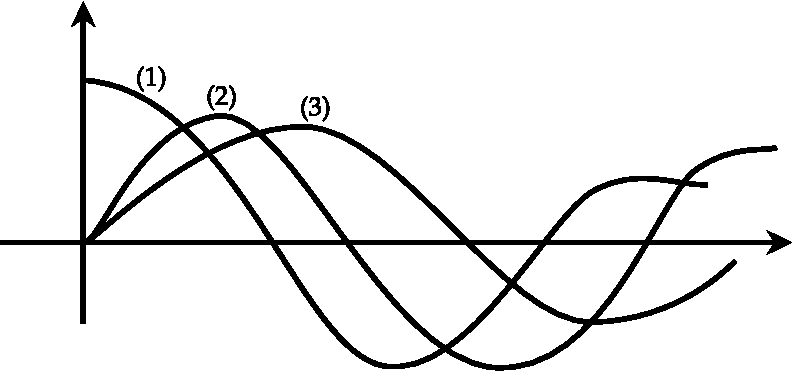
\includegraphics[height=3.5cm,width=6.5cm]{SF-01}
\end{figure}
 \begin{tasks}(2)
	\task[\textbf{a.}](1) $J_{0}$,
	(2) $J_{2}$, (3) $J_{1}$
	\task[\textbf{b.}]$(1) J_{0}$,
	(2) $J_{1}, \quad(3) J_{2}$
	\task[\textbf{c.}](1) $J_{2}$,
	(2) $J_{1}$,
	(3) $J_{0}$
	\task[\textbf{d.}] None of the above
\end{tasks}
\begin{answer}
	So the correct answer is \textbf{Option (b)}
\end{answer}
\item If the generating function of Legendre polynomial is $\frac{1}{\sqrt{1-6 t+t^{2}}}$, then coefficient of $t^{2}$ is
 \begin{tasks}(4)
	\task[\textbf{a.}] 11
	\task[\textbf{b.}]$-11$
	\task[\textbf{c.}]13
	\task[\textbf{d.}] $-13$
\end{tasks}
\begin{answer}
	\begin{align*}
	\intertext{The generating function for the polynomial solutions of the Legendre ODE is given by}
	g(x, t)&=\frac{1}{\sqrt{1-2 x t+t^{2}}}=\sum_{n=0}^{\infty} P_{n}(x) t^{n}\\
	\text{Thus }x&=3\text{ and }n=2.\\
	P_{2}(x)&=\frac{1}{2}\left(3 x^{2}-1\right) \Rightarrow P_{2}(3)=\frac{1}{2}\left(3 \times 3^{2}-1\right)=13
	\end{align*}
		So the correct answer is \textbf{Option (c)}
\end{answer}
\item Which of the following relation is true for Bessel's differential equation?
 \begin{tasks}(2)
	\task[\textbf{a.}]$J_{0}^{\prime}(x)=J_{1}(x)$
	\task[\textbf{b.}]$J_{0}^{\prime}(x)=-J_{2}(x)$
	\task[\textbf{c.}]$J_{0}^{\prime}(x)=J_{2}(x)$
	\task[\textbf{d.}] $J_{0}^{\prime}(x)=-J_{1}(x)$
\end{tasks}
\begin{answer}
	So the correct answer is \textbf{Option (d)}
\end{answer}
\item Given that $\sum_{n=0}^{\infty} H_{n}(x) \frac{t^{n}}{n !}=e^{-t^{2}+2 x x}$ the value of $H_{6}(0)$ is
 \begin{tasks}(4)
	\task[\textbf{a.}]$-120$
	\task[\textbf{b.}]$+120$
	\task[\textbf{c.}]12
	\task[\textbf{d.}]  $-12$
\end{tasks}
\begin{answer}
	\begin{align*}
	\sum_{n=0}^{\infty} I_{n}(x) \frac{t^{\prime \prime}}{n !}&=e^{-t^{2}+2 t x} \Rightarrow \sum_{n=0}^{\infty} H_{n}(0) \frac{t^{n}}{n !}=e^{-t^{2}}=1-t^{2}+\frac{t^{4}}{2 !}-\frac{t^{6}}{3 !}\\
	\Rightarrow \frac{H_{6}(0)}{6 !} t^{6}&=-\frac{1}{3 !} t^{6} \Rightarrow H_{6}(0)=-\frac{6 !}{3 !}=-120
	\end{align*}
	So the correct answer is \textbf{Option (a)}
\end{answer}
\item Given that $\sum_{n=0}^{\infty} H_{n}(x) \frac{t^{n}}{n !}=e^{-t^{2}+2 e x}$ the value of $H_{4}(0)$ is
 \begin{tasks}(4)
	\task[\textbf{a.}]12
	\task[\textbf{b.}] 6
	\task[\textbf{c.}]24
	\task[\textbf{d.}] $-6$
\end{tasks}
\begin{answer}
	\begin{align*}
	\sum_{n=0}^{\infty} H_{n}(x) \frac{t^{n}}{n !}&=e^{-t^{2}+2 t x} \Rightarrow \sum_{n=0}^{\infty} H_{n}(0) \frac{t^{n}}{n !}=e^{-t^{2}}=1-t^{2}+\frac{t^{4}}{2 !}-\frac{t^{6}}{3 !}\\
	\Rightarrow \frac{H_{4}(0)}{4 !} t^{4}&=\frac{t^{4}}{2 !} \Rightarrow H_{4}(0)=\frac{4 !}{2 !}=12
	\end{align*}
	So the correct answer is \textbf{Option (a)}
\end{answer}
\item If Hermite polynomial of order 2 is given by $H_{2}(x)=a x^{2}-2 ; a>0$, then the value of $a$ is
 \begin{tasks}(4)
	\task[\textbf{a.}]3
	\task[\textbf{b.}]4
	\task[\textbf{c.}]5
	\task[\textbf{d.}] 6
\end{tasks}
\begin{answer}
	\begin{align*}
	\intertext{Orthonormality condition,}
	\int_{-\infty}^{+\infty}\left[H_{n}(x)\right]^{2} e^{-x^{2}} d x&=2^{\prime \prime} n ! \sqrt{\pi}\\
	\text{For, }n&=2, \int_{-\infty}^{+\infty}\left(a x^{2}-2\right)^{2} e^{-x^{2}} d x=8 \sqrt{\pi}\\
\text{	Now}
	\int_{-\infty}^{+\infty}\left[H_{2}(x)\right]^{2} e^{-x^{2}} d x&=\int_{-\infty}^{+\infty}\left(a x^{2}-2\right)^{2} e^{-x^{2}} d x=\left\{a^{2} \times \frac{3}{4}+4-2 a\right\} \sqrt{\pi}
	\intertext{Thus, we have}
	\frac{3 a^{2}}{4}+4-2 a&=8 \Rightarrow 3 a^{2}-8 a-16=0 \Rightarrow 3 a^{2}-12 a+4 a-16=0\\
	\Rightarrow 3 a(a-4)+4(a-4)&=0 \Rightarrow(3 a+4)(a-4)=0\\
	\text{Thus, }a&=4
	\end{align*}
		So the correct answer is \textbf{Option (b)}
\end{answer}
\item The value of Legendre polynomial $p_{n}(x)$ for odd $n$ and $x=0$. i.e., $p_{n}(0)$ is
 \begin{tasks}(4)
	\task[\textbf{a.}]1
	\task[\textbf{b.}]0
	\task[\textbf{c.}]$-1$
	\task[\textbf{d.}]  $0.5$
\end{tasks}
\begin{answer}
	\begin{align*}
	\intertext{The generating function for Legendre polynomial is}
	\left(1-2 x t+t^{2}\right)^{-1 / 2}&=\sum_{n=0}^{\infty} p_{n}(x) t^{n}\\
	\text{Put, $x=0$, we get, }&\left(1+t^{2}\right)^{-1 / 2}=\sum p_{n}(\theta) t^{n}
	\end{align*}
		So the correct answer is \textbf{Option (b)}
\end{answer}
\item For the Legendre's polynomial $P_{n}(x)$, given below are two statements. Study these carefully and pick out the correct option.\\
Statement I: $\quad \int_{-1}^{1} x\left[P_{n}(x)\right]^{2} d x=0$\\
Statement I: $\lim _{n \rightarrow \infty}\left[\int_{-1}^{1} x P_{n}(x) P_{n+1}(x) d x\right]=0$
 \begin{tasks}(1)
	\task[\textbf{a.}]Only statement (I) is correct
	\task[\textbf{b.}]Only statement (II) is correct
	\task[\textbf{c.}]Both (I) and (II) are correct
	\task[\textbf{d.}]Neither (I) nor (II) is correet
\end{tasks}
\begin{answer}
	\begin{align*}
	\intertext{From recurrence relation we have}
	(n+1) P_{n+1}(x)&=(2 n+1) x p_{n}(x)-n p_{n-1}(x)\\
	x p_{n}(x)&=\frac{1}{(2 n+1)}\left\{(n+1) p_{n+1}(x)+n p_{n-1}(x)\right\}\\
	x\left[p_{n}(x)\right]^{2}&=\frac{1}{(2 n+1)}\left\{(n+1) p_{n}(x) p_{n+1}(x)+n p_{n}(x) p_{n-1}(x)\right\}\\
	\therefore \int_{-1}^{+1} x\left[p_{n}(x)\right]^{2} d x&=0\left\{\because \int_{-1}^{+1} p_{m}(x) p_{n}(x)=0\right.\text{ if }\left.m \neq n\right\}\\
	\therefore &\int_{-1}^{+1} x\left[p_{n}(x)\right]^{2} d x=0
	\intertext{From recurrence relation, we have}
	(n+1) p_{n+1}(x)&=(2 n+1) x p_{n}(x)-n p_{n-1}(x)\\
	(2 n+1) x p_{n}(x)&=(n+1) p_{n+1}(x)+n p_{n-1}(x)\\
	\int_{-1}^{+1}(2 n+1) x p_{n}(x) p_{n+1}(x) d x&=\int_{-1}^{+1}\left[(n+1)\left\{p_{n+1}(x)\right\}^{2}+n p_{n-1}(x) p_{n+1}(x)\right] d x\\
	=\int_{-1}^{+1}(n+1)\left\{p_{n+1}(x)\right\}^{2} d x+n \int_{-1}^{+1}& p_{n-1}(x) p_{n+1}(x) d x=(n+1) \frac{2}{2(n+1)+1}+0=\frac{2 n+2}{2 n+3}\\
	\therefore \int_{-1}^{+1} x p_{n}(x) p_{n+1}(x) d x&=\frac{2 n+2}{(2 n+1)(2 n+3)}\\
	\lim _{n \rightarrow \infty} \frac{n\left(2+\frac{2}{n}\right)}{n^{2}\left(2+\frac{1}{n}\right)\left(2+\frac{3}{n}\right)}&=\lim _{n \rightarrow \infty} \frac{\left(2+\frac{2}{n}\right)}{n\left(2+\frac{1}{n}\right)\left(2+\frac{3}{n}\right)}=0
	\end{align*}
		So the correct answer is \textbf{Option (c)}
\end{answer}
\item Which of the following statements is Incorrect about the Hermite polynomials $H_{n}(x)$ ?
 \begin{tasks}(1)
	\task[\textbf{a.}] The value of integral $\frac{1}{\sqrt{\pi}} \int_{-\infty}^{\infty} e^{-x^{2}}\left[H_{4}(x)\right]^{2} d x$ is 384
	\task[\textbf{b.}] Hermite polynomial of order $3, H_{3}(x)$, satisfies the differential equation $y^{\prime \prime}-2 x y^{\prime}+6 y=0$
	\task[\textbf{c.}] The value of $\mathrm{H}_{4}(\mathrm{l})$ is $-20$
	\task[\textbf{d.}] $H_{n}(x)=\frac{H_{n+1}(x)+2 n H_{n-1}(x)}{x}$
\end{tasks}
\begin{answer}
	\begin{align*}
	\intertext{When integrated with respect to weight function $e^{-x^{2}}$, the Hermite polynomials satisfy}
	\int_{-\infty}^{\infty} e^{-x^{2}} H_{n}(x) H_{m}(x) d x&= \begin{cases}0, & n \neq m \\ \sqrt{\pi} 2^{n} n !, & n=m\end{cases}
	\intertext{In our case $n=m=4$, hence}
	\frac{1}{\sqrt{\pi}} \int_{-\infty}^{\infty} e^{-x^{2}}\left[H_{4}(x)\right]^{2} d x&=\frac{\sqrt{\pi} 2^{4}(4 !)}{\sqrt{\pi}}=384
	\intertext{Hermite polynomial of order $n$, satisfies the differential equation}
	y^{\prime \prime}-2 x y^{\prime}+2 n y=0\\
\text{	when }n=3, y^{\prime \prime}-2 x y^{\prime}+6 y=0\\
	\text{We have }H_{4}(x)&=16 x^{4}-48 x^{2}+12\\
	\text{Therefore, }H_{4}(1)&=-48+28=-20
	\intertext{The recursion relation for Hermite polynomials is}
	H_{n+1}(x)&=2 x H_{n}(x)-2 n H_{n-1}(x) \Rightarrow H_{n}(x)=\frac{H_{n+1}(x)+2 n H_{n-1}(x)}{2 x}
	\end{align*}
		So the correct answer is \textbf{Option (d)}
\end{answer}
\item If $P_{n}(x)$ denotes the Legendre polynomials of order $n$, then which of the following statements is incorrect?
 \begin{tasks}(1)
	\task[\textbf{a.}]$P_{n}(x)=\frac{1}{2^{n} n !} \frac{d^{n}}{d x^{n}}\left[\left(x^{2}-1\right)^{n}\right]$ where $n=0,1,2 \ldots$
	\task[\textbf{b.}]The Legendre polynomials satisfy the differential equation\\$
	\left(1-x^{2}\right) \frac{d^{2} y}{d x^{2}}-2 x \frac{d y}{d x}+n(n+1) y=0
	$
	\task[\textbf{c.}] For each value of $n$ the Legendre polynomials satisfy the relation $P_{n}(1)=1$.
	\task[\textbf{d.}] The value of integral $\int_{-1}^{1}\left[P_{4}(x)\right]^{2} d x$ is $\frac{2}{7}$.
\end{tasks}
\begin{answer}
	\begin{align*}
	\intertext{Option (a) is the correct definition of Legendre polynomial. Legendre polynoimials satisfy the differential equation given in option (b). For each value of $n$ Legendre polynomials satisfy $P_{n}(1)=1$.}
	\text{Since, }\int_{-1}^{1}\left[P_{n}(x)\right]^{2} d x&=\frac{2}{2 n+1}\\
	\text{Hence, }\int_{-1}^{1}\left[P_{4}(x)\right]^{2} d x&=\frac{2}{2 \cdot 4+1}=\frac{2}{9}\\
	\text{Hence option }&(d)\text{ is incorrect.}
	\end{align*}
		So the correct answer is \textbf{Option (d)}
\end{answer}
\end{enumerate}
%\chapter{Fourier Transform}
\begin{enumerate}
	\item Let $F(k)$ is the Fourier exponential transform of $f(x)$ and $G(k)$ be the Fourier Transform of $g(x)=f(x+a)$. Then $G(k)$ is given by
	(Use the Fourier integral $F(k)=\frac{1}{\sqrt{2 \pi}} \int_{-\infty}^{+\infty} f(x) e^{i k x} d x$ )
	 \begin{tasks}(2)
		\task[\textbf{a.}]$e^{i a k} f(k)$
		\task[\textbf{b.}]$e^{-i a k} F(-k)$
		\task[\textbf{c.}] $e^{-i a k} F(k)$
		\task[\textbf{d.}] $e^{-i a k} f(k)$
	\end{tasks}
	\item The value of a function is given by $f(x)=\left\{\begin{array}{cc}1 & 0<x<1 \\ -1 & 1<x<2 \\ 0 & x>2\end{array}\right.$, the Fourier cosine transform of $f(x)$ is
	 \begin{tasks}(2)
		\task[\textbf{a.}]$\sqrt{\frac{2}{\pi}}\left(\frac{2 \sin \omega+\sin 2 \omega}{\omega}\right)$
		\task[\textbf{b.}]$\sqrt{\frac{2}{\pi}}\left(\frac{2 \sin \omega-\sin 2 \omega}{\omega}\right)$
		\task[\textbf{c.}]$\sqrt{\frac{2}{\pi}}\left(\frac{\sin \omega-\sin 2 \omega}{\omega}\right)$
		\task[\textbf{d.}] $\sqrt{\frac{2}{\pi}}\left(\frac{2 \sin \omega}{\omega}\right)$
	\end{tasks}
	\item Consider the function $\delta_{n}(x)=\frac{n}{\sqrt{\pi}} \exp \left(-n^{2} x^{2}\right)$. For $n \rightarrow \infty$ The Fourier transform of the function is given by
	 \begin{tasks}(2)
		\task[\textbf{a.}]$\delta(x)=\int_{-\infty}^{+\infty} e^{-i k x} d k$
		\task[\textbf{b.}]$\delta(x)=\frac{1}{2 \pi} \int_{-\infty}^{+\infty} e^{i k x} d k$
		\task[\textbf{c.}]$\delta(x)=\frac{1}{2 \pi} \int_{-\infty}^{+\infty} e^{-i k x} d k$
		\task[\textbf{d.}] 0
	\end{tasks}
	\item For the function $f(t)=\delta(t-x)$, the Fourier cosine integral is defined as $g_{c}(\omega)=\sqrt{\frac{2}{\pi}} \int_{0}^{\infty} f(t) \cos \omega t d t$. Its Fourier transform is:
	 \begin{tasks}(2)
		\task[\textbf{a.}] $\sqrt{\frac{2}{\pi}} \cos \omega x$
		\task[\textbf{b.}]$\sqrt{\frac{2}{\pi}}$
		\task[\textbf{c.}]$\sqrt{\frac{2}{\pi}} \sin \omega x$
		\task[\textbf{d.}] $i \sqrt{\frac{2}{\pi}}$
	\end{tasks}
	\item Inverse cosine transform of $g_{c}(\omega)=\sqrt{\frac{2}{\pi}} \cos \omega x$ is:
	 \begin{tasks}(2)
		\task[\textbf{a.}]$\delta(t+x)$
		\task[\textbf{b.}]$\delta(t-x)$
		\task[\textbf{c.}]$\delta(t-x)(t+x)$
		\task[\textbf{d.}] $\delta^{2}(x-t)(x+t)$
	\end{tasks}
	\item $f(t)=\frac{\hbar}{2 \pi i} \int_{-\infty}^{+\infty} \frac{e^{-i \omega t} d \omega}{\left(E_{0}-i \Gamma / 2-\hbar \omega\right)}$ The value of $f(t)$ is given by
	 \begin{tasks}(2)
		\task[\textbf{a.}](a) $f(t)= \begin{cases}e^{-\Gamma t / 2 \hbar} e^{-i E_{0} t / \hbar} & , t>0 \\ 0 & , t<0\end{cases}$
		\task[\textbf{b.}]$f(t)= \begin{cases}e^{\sqrt{1 / 2 \hbar}} e^{-1 E_{0} t / \hbar} & , t>0 \\ 0 & , t<0\end{cases}$
		\task[\textbf{c.}]$f(t)= \begin{cases}e^{-\Gamma t / 2 \hbar} e^{-i E_{0} t / \hbar} & , t>0 \\ 0 & , t<0\end{cases}$
		\task[\textbf{d.}] $f(t)= \begin{cases}e^{-\Gamma t / 2 h} e^{-i E_{0} t / h} & , t>0 \\ e^{-i E_{0} t / \hbar} & , t<0\end{cases}$
	\end{tasks}
	\item The Fourier transform of function $h(t)=t e^{-t^{2}}$ is 
	 \begin{tasks}(2)
		\task[\textbf{a.}] $j \pi f e^{-\pi^{2} f^{2}}$
		\task[\textbf{b.}]$-j \pi f e^{-\pi^{2} f^{2}}$
		\task[\textbf{c.}]$j \pi f e^{-\pi^{2} f^{2} / 4}$
		\task[\textbf{d.}] $-j \pi f e^{-\pi^{2} f^{2} / 4}$
	\end{tasks}
	\item The graph of a real periodic function $f(x)$ for the range $[-\infty, \infty]$ is shown below
	\begin{figure}[H]
		\centering
		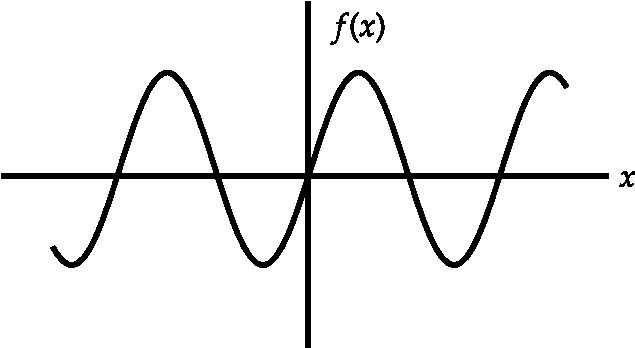
\includegraphics[height=3cm,width=5cm]{FT-Assignment-05}
	\end{figure}
	Which of the following graphs represents the real part of its Fourier transform?
	 \begin{tasks}(2)
		\task[\textbf{a.}]	
		\begin{figure}[H]
			\centering
			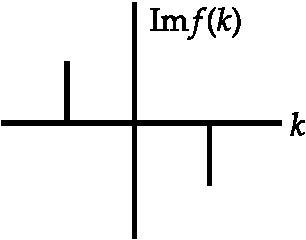
\includegraphics[height=2.2cm,width=3cm]{FT-Assignment-01}
		\end{figure}
		\task[\textbf{b.}]
			\begin{figure}[H]
			\centering
			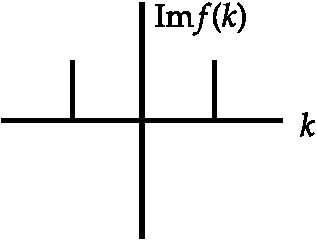
\includegraphics[height=2.2cm,width=3cm]{FT-Assignment-02}
		\end{figure}
		\task[\textbf{c.}]
			\begin{figure}[H]
			\centering
			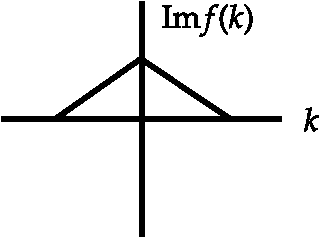
\includegraphics[height=2.2cm,width=3cm]{FT-Assignment-03}
		\end{figure}
		\task[\textbf{d.}] 
			\begin{figure}[H]
			\centering
			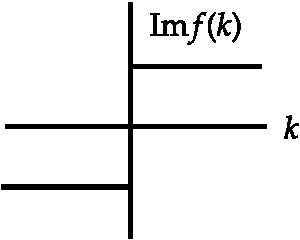
\includegraphics[height=2.2cm,width=3cm]{FT-Assignment-04}
		\end{figure}
	\end{tasks}
	\item The Fourier transform of the function $h(t)=\left\{\begin{array}{cc}\beta e^{-a t}, & t>0 \\ 0, & t<0\end{array}\right.$, is given by
	 \begin{tasks}(2)
		\task[\textbf{a.}]$H(f)=\frac{\alpha}{\sqrt{\alpha^{2}+(2 \pi f)^{2}}} e^{j \tan ^{-1}\left[-2 \pi f^{\prime \alpha]}\right.}$
		\task[\textbf{b.}]$H(f)=\frac{\beta}{\sqrt{\alpha^{2}+(2 \pi f)^{2}}} e^{j \tan ^{-1}[-2 \pi f / \beta]}$
		\task[\textbf{c.}]$H(f)=\frac{\beta}{\sqrt{\alpha^{2}+(2 \pi f)^{2}}} e^{\tan ^{-1}[2 \pi f / \alpha]}$
		\task[\textbf{d.}] $H(f)=\frac{\beta}{\sqrt{\alpha^{2}+(2 \pi f)^{2}}} e^{j \tan ^{-1}[-2 \pi f / \alpha]}$
	\end{tasks}
	\item The Fourier transform of $f(x)=\left\{\begin{array}{cl}-1 & -1<x<0 \\ 1 & 0<x<1 \\ 0 & \text { otherwise }\end{array}\right.$ is
	 \begin{tasks}(2)
		\task[\textbf{a.}] $\frac{i}{\omega} \sqrt{\frac{2}{\pi}}(\cos \omega+1)$
		\task[\textbf{b.}] $\frac{i}{\omega} \sqrt{\frac{2}{\pi}}(\cos \omega-1)$
		\task[\textbf{c.}]$-\frac{i}{\omega} \sqrt{\frac{2}{\pi}}(1+\cos \omega)$
		\task[\textbf{d.}] $\frac{i}{\omega} \sqrt{\frac{2}{\pi}}(1-\cos \omega)$
	\end{tasks}
	\item The Fourier transform of $f(x)= \begin{cases}x, & 0<x<a \\ 0, & \text { otherwise }\end{cases}$ is
	 \begin{tasks}(2)
		\task[\textbf{a.}]$\frac{1}{\sqrt{2 \pi} \cdot \omega^{2}}\left[e^{-i \omega n a}(1+i a \omega)-1\right]$
		\task[\textbf{b.}]$\frac{1}{\sqrt{2 \pi} \cdot \omega^{2}}\left[e^{-i \omega a}(1-i a \omega)-1\right]$
		\task[\textbf{c.}] $\frac{1}{\sqrt{2 \pi} \cdot \omega^{2}}\left[e^{-1 \text { tox }}(1+i a \omega)+1\right]$
		\task[\textbf{d.}] $\frac{1}{\sqrt{2 \pi} \cdot \omega^{2}}\left[e^{-i \omega a}(1-i a \omega)+1\right]$
	\end{tasks}
	
	
	
	
	
	
\end{enumerate}
%\chapter{Fourier Transform}
\begin{enumerate}
	\item  $\left. \right. $
	\begin{answer}
		\begin{align*}
		F(k)&=\frac{1}{\sqrt{2 \pi}} \int_{-\infty}^{+\infty} f(x) e^{i k x} d x\\
		\because g(x)&=f(x+a)\\
		\therefore G(k)&=\frac{1}{\sqrt{2 \pi}} \int_{-\infty}^{+\infty} f(x+a) e^{i k x} d x\\
		\text{Let }x+a&=y, d x=d y\\
		\therefore G(k)&=\frac{1}{\sqrt{2 \pi}} \int_{-\infty}^{+\infty} f(y) e^{i k(y-a)} d y=e^{-i k a} \frac{1}{\sqrt{2 \pi}} \int_{-\infty}^{+\infty} f(x) e^{i k x} d x=e^{-i a k} F(k)
	\end{align*}
		So the correct answer is \textbf{Option (c)}
	\end{answer}
	\item  $\left. \right. $
	\begin{answer}
		\begin{align*}
		 f_{c}(\omega) &=\sqrt{\frac{2}{\pi}} \int_{0}^{\infty} f(x) \cos \omega x d x \\ &=\sqrt{\frac{2}{\pi}} \int_{0}^{1} \cos \omega x d x+\sqrt{\frac{2}{\pi}} \int_{1}^{2}-\cos \omega x d x \\ &=\sqrt{\frac{2}{\pi}}\left[\left(\frac{\sin \omega x}{\omega}\right)_{0}^{1}-\left(\frac{\sin \omega x}{\omega}\right)_{1}^{2}\right] \\ &=\sqrt{\frac{2}{\pi}}\left(\frac{2 \sin \omega-\sin 2 \omega}{\omega}\right) 
		\end{align*}
		So the correct answer is \textbf{Option (b)}
	\end{answer}
	\item  $\left. \right. $
	\begin{answer}
		\begin{align*}
		\mathrm{n}: g(k)&=\frac{1}{\sqrt{2 \pi}} \int_{-\infty}^{+\infty} \frac{n}{\sqrt{\pi}} e^{-n^{2} x^{2}} e^{i k x} d x=\frac{n}{\sqrt{2} \cdot \pi} \int_{-\infty}^{+\infty} e^{-n^{2} x^{2}+i i x} d x=\frac{n}{\sqrt{2} \cdot \pi} e^{-k^{2} / 4 n^{2}} \int_{-\infty}^{+\infty} e^{-n^{2}\left(x-\frac{i k}{2 n^{2}}\right)^{2}} d x\\
		&=\frac{n}{\sqrt{2} \cdot \pi} e^{-k^{2} / 4 n^{2}} \times 2 \times \frac{1}{2} \cdot \frac{\sqrt{\pi}}{n}=\frac{1}{\sqrt{2 \pi}} e^{-k^{2} / 4 n^{2}}
		\intertext{ Now inverse fourier transform of $g(k)$ is}
		\delta_{n}(x)&=\frac{1}{\sqrt{2 \pi}} \int_{-\infty}^{+\infty} \frac{e^{-k^{2} / 4 n^{2}}}{\sqrt{2 \pi}} \cdot e^{-i k x} d k\\
		\delta(x)&=\lim _{n \rightarrow \infty} \delta_{n}(x)=\lim _{n \rightarrow \infty} \frac{1}{2 \pi} \int_{-\infty}^{+\infty} e^{-k^{2} / 4 n^{2}} \cdot e^{-i k x} d k=\frac{1}{2 \pi} \int_{-\infty}^{+\infty} e^{-i k x} d k\\
		\therefore \delta(x)&=\frac{1}{2 \pi} \int_{-\infty}^{+\infty} e^{-i k x} d k
		\end{align*}
		So the correct answer is \textbf{Option (c)}
	\end{answer}
	\item  $\left. \right. $	
	\begin{answer}
		\begin{align*}
		\text{(i) }g_{c}(\omega)=\sqrt{\frac{2}{\pi}} \int_{0}^{\omega} \delta(t-x) \cos \omega t d t=\sqrt{\frac{2}{\pi}} \cos \omega x
		\end{align*}
		So the correct answer is \textbf{Option (a)}
	\end{answer}
		\item  $\left. \right. $	
	\begin{answer}
		\begin{align*}
		f(t)&=\delta(t-x)=\sqrt{\frac{2}{\pi}} \int_{0}^{+\infty} \sqrt{\frac{2}{\pi}} \cos \omega x \cos \omega t d \omega\\
		\Rightarrow \delta(t-x)&=\frac{2}{\pi} \int_{0}^{\infty} \cos \omega t \cos \omega x d \omega
		\end{align*}
		So the correct answer is \textbf{Option (b)}
	\end{answer}
		\item  $\left. \right. $
	\begin{answer}
		\begin{align*}
		\intertext{Fourier Transform of $f(t)$ is}
		g(\omega)&=\frac{1}{\sqrt{2 \pi}} \int_{0}^{\infty} e^{-\Gamma t / 2 \hbar} \cdot e^{-i E_{0} / / \hbar} \cdot e^{i a t} d t=\frac{1}{\sqrt{2 \pi}} \int_{0}^{\infty} \exp \left\{\frac{-i t}{\hbar}\left(E_{0}-i \Gamma / 2-\hbar \omega\right)\right\} d t\\
		&=\frac{1}{\sqrt{2 \pi}}\left[\frac{e^{\left\{\frac{-i t}{\hbar}\left(E_{0}-i / / 2-\hbar \omega\right)\right\}}}{\frac{-i}{\hbar}\left(E_{0}-i \Gamma / 2-\hbar \omega\right)}\right]_{0}^{\infty}=\frac{1}{\sqrt{2 \pi}}\left[\frac{0-1}{\frac{-i}{\hbar}\left(E_{0}-i \Gamma / 2-\hbar \omega\right)}\right]\\
		&=\frac{1}{\sqrt{2 \pi} i(E o-i \Gamma / 2-h \omega)}
		\intertext{Inverse transform of $g(\omega)$ is}
		f(t)&=\frac{1}{2 \pi} \int_{-\infty}^{+\infty} \frac{\hbar e^{-i \omega x}}{i\left(E_{0}-i \Gamma / 2-\hbar \omega\right)} d \omega=\frac{\hbar}{2 \pi i} \int_{-\infty}^{+\infty} \frac{e^{-i \omega t} d \omega}{\left(E_{0}-i \Gamma / 2-\hbar \omega\right)}\\
		\therefore &\frac{\hbar}{2 \pi i} \int_{-\infty}^{+\infty} \frac{e^{-i \omega t} d \omega}{\left(E_{0}-i \Gamma / 2-\hbar \omega\right)}=f(t)= \begin{cases}\exp (-\Gamma t / 2 \hbar) \exp \left(\frac{-i E_{0} t}{\hbar}\right), & t>0 \\ 0 & t<0\end{cases}
		\end{align*}
		So the correct answer is \textbf{Option (c)}
	\end{answer}
	\item  $\left. \right. $
	\begin{answer}
		\begin{align*}
		F\left\{t e^{-r^{2}}\right\}&=-\frac{1}{2} F\left\{\frac{d\left(e^{-r^{2}}\right)}{d t}\right\}=-\frac{1}{2}(j 2 \pi f) F\left\{e^{-t^{2}}\right\}=-j \pi f e^{-\pi^{2} f^{2}}
		\end{align*}
		So the correct answer is \textbf{Option (b)}
	\end{answer}
		\item  $\left. \right. $
	\begin{answer}
		\begin{align*}
		\intertext{This is sine function}
		f(x)&=A \sin x \Rightarrow F(k)=j \frac{A}{2}\left[\delta\left(k-k_{0}\right)-\delta\left(k+k_{0}\right)\right]
		\end{align*}
		So the correct answer is \textbf{Option (a)}
	\end{answer}
		\item  $\left. \right. $
	\begin{answer}
		\begin{align*}
		H(f)&=\int_{-\infty}^{+\infty} h(t) e^{-j 2 \pi f t} d t=\int_{0}^{+\infty} \beta e^{-\alpha t} e^{-j 2 \pi f t} d t=\beta \int_{0}^{+\infty} e^{-(\alpha+j 2 \pi f) t} d t\\
		\Rightarrow H(f)&=\left.\frac{-\beta}{\alpha+j 2 \pi f} e^{-(\alpha+j 2 \pi f) t}\right|_{0} ^{\infty}=\frac{\beta}{\alpha+j 2 \pi f}=\frac{\beta \alpha}{\alpha^{2}+(2 \pi f)^{2}}-j \frac{2 \pi f \beta}{\alpha^{2}+(2 \pi f)^{2}}\\
		\Rightarrow H(f)&=\frac{\beta}{\sqrt{\alpha^{2}+(2 \pi f)^{2}}} e^{j \tan ^{-1}[-2 \pi f / \alpha]}
		\end{align*}
		So the correct answer is \textbf{Option (d)}
	\end{answer}
		\item  $\left. \right. $
	\begin{answer}
		\begin{align*}
		f(x)&=\left\{\begin{array}{rl}-1 & -1<x<0 \\ 1 & 0<x<1 \\ 0 & \text { otherwise }\end{array}\right.\\
		F[f(x)]&=\frac{1}{\sqrt{2 \pi}}\left[\int_{-1}^{0}-e^{-i \omega x} d x+\int_{0}^{1} e^{-i \omega x} d x\right]\\
		&=\frac{1}{\sqrt{2 \pi}}\left[-\left(\frac{e^{-i \omega x}}{-i \omega}\right)_{-1}^{0}+\left(\frac{e^{-i \omega x}}{-i \omega}\right)_{0}^{1}\right]=\frac{1}{\sqrt{2 \pi}}\left[\frac{-1+e^{i \omega}}{-i \omega}+\frac{e^{-i \omega}-1}{-i \omega}\right]\\
		&=\frac{1}{\sqrt{2 \pi}}\left[\frac{2 \cos \omega-2}{-i \omega}\right]=\frac{i}{\omega} \sqrt{\frac{2}{\pi}}(\cos \omega-1)
		\end{align*}
		So the correct answer is \textbf{Option (b)}
	\end{answer}
		\item  $\left. \right. $
		\begin{answer}
			\begin{align*}
			f(x)&= \begin{cases}x, & 0<x<a \\ 0, & \text { otherwise }\end{cases}\\
			F[f(x)]&=\frac{1}{\sqrt{2 \pi}} \int_{0}^{a} x e^{-i \omega x} d x=\frac{1}{\sqrt{2 \pi}}\left[\left(\frac{x e^{-i e x}}{-i \omega}\right)_{0}^{a}-\left(\frac{e^{-i \omega x}}{(-i \omega)^{2}}\right)_{0}^{a}\right]\\&=\frac{1}{\sqrt{2 \pi}}\left[\frac{a e^{-i \omega a}}{-i \omega}-\frac{e^{-i \omega a}-1}{(-i \omega)^{2}}\right]=\frac{1}{\sqrt{2 \pi}}\left[\frac{i a \omega e^{-i e a}}{\omega^{2}}+\frac{e^{-i e a}-1}{\omega^{2}}\right]\\
			&=\frac{1}{\sqrt{2 \pi} \cdot \omega^{2}}\left[e^{-i \omega x}(1+i a \omega)-1\right]
			\end{align*}
			So the correct answer is \textbf{Option (a)}
		\end{answer}
\end{enumerate}
%\chapter{Laplace Transforms}
The Laplace transform $f(s)$ of a function $F(t)$ is defined by 
\begin{equation}
f(s)=\mathcal{L}\{F(t)\}=\int_{0}^{\infty} e^{-s t} F(t) d t .
\end{equation}
A few comments on the existence of the integral are in order. The infinite integral of $F(t)$,
\begin{equation*}
\int_{0}^{\infty} F(t) d t,
\end{equation*}
need not exist. For instance, $F(t)$ may diverge exponentially for large $t$. However, if there are some constants $s_{0}, M$, and $t_{0} \geq 0$ such that for all $t>t_{0}$
\begin{equation}
\left|e^{-s_{0} t} F(t)\right| \leq M,\label{LT-01}
\end{equation}
the Laplace transform will exist for $s>s_{0} ; F(t)$ is then said to be of exponential order. As a counterexample, $F(t)=e^{t^{2}}$ does not satisfy the condition given by Eq. (\ref{LT-01}) and is not of exponential order. Thus, $\mathcal{L}\left\{e^{t^{2}}\right\}$ does not exist.

The Laplace transform may also fail to exist because of a sufficiently strong singularity in the function $F(t)$ as $t \rightarrow 0$. For example,
\begin{equation*}
\int_{0}^{\infty} e^{-s t} t^{n} d t
\end{equation*}
diverges at the origin for $n \leq-1$. The Laplace transform $\mathcal{L}\left\{t^{n}\right\}$ does not exist for $n \leq-1$. Since, for two functions $F(t)$ and $G(t)$ for which the integrals exist,
\begin{equation}
\mathcal{L}\{a F(t)+b G(t)\}=a \mathcal{L}\{F(t)\}+b \mathcal{L}\{G(t)\}
\end{equation}
the operation denoted by $\mathcal{L}$ is linear.\\
$\textbf{Important Laplace Transforms:}$\\
\renewcommand*{\arraystretch}{2}
\begin{tabular}{p{6cm}p{6cm}}
	(1) $L(1)=\frac{1}{s}$&
(2) $L\left(x^{n}\right)=\frac{n !}{s^{n+1}}(n=0,1,2, \ldots \ldots . .)$\\
(3) $L\left(e^{a x}\right)=\frac{1}{s-a}(s>a)$&
(4) $L(\cos a x)=\frac{s}{s^{2}+a^{2}}$
$(s>0)$\\
(5) $L(\sin a x)=\frac{a}{s^{2}+a^{2}} \quad(s>0)$&
(6) $L(\cosh a x)=\frac{s}{s^{2}-a^{2}}\left(s^{2}>a^{2}\right)$\\
(7) $L(\sinh a x)=\frac{a}{s^{2}-a^{2}}\left(s^{2}>a^{2}\right)$.& 
\end{tabular}
\textbf{Important properties:}\\
\begin{enumerate}
	\item Linear Property: $L\left[a_{1} f_{1}(x)+a_{2} f_{2}(x)\right]=a_{1} L\left[f_{1}(x)\right]+a_{2} L\left[f_{2}(x)\right]$
	\item Shifting Property: $L\left[e^{a x} f(x)\right]=f(s-a)$
	\item Scaling Property: $L[f(a x)]=\frac{1}{a} f\left(\frac{s}{a}\right)$
	\item $L\left[x^{n} f(x)\right]=(-1)^{n} \frac{d^{n}}{d s^{n}}(f(s))$
	\item $L\left[\frac{f(x)}{x}\right]=\int_{-\infty}^{\infty} f(s) d s$
	\item $L\left[\int_{0}^{t} f(x) d x\right]=\frac{1}{s} f(s)$
	\item $L\left[f^{\prime}(x)\right]=s L[f(x)]-f(0)$
	\item  $L\left[f^{\prime \prime}(x)\right]=s^{2} L[f(x)]-f^{\prime}(0)-s f(0)$
	\item Laplace transform of a periodic function $f(x)$ having period ' $T$ ' is\\$L[f(\dot{x})]=\frac{1}{1-e^{-s T}} \int_{0}^{T} e^{-s x} f(\dot{x}) d \dot{x}$
	\item Laplace transform of the unit step function $u(x-a)=u_{a}(x)=\left\{\begin{array}{lll}0 & \text { for } & x<a \\ 1 & \text { for } & x \geq a\end{array}\right.$ is $\frac{e^{-a s}}{s}$.
	\item Laplace transform of the dirac delta function $\delta(x-a)$ is $e^{-a s}$.
\end{enumerate}
\begin{exercise}
	Find the laplace transform of $f(x)=(1+\cos 2 x)$
\end{exercise}
\begin{answer}
	\begin{align*}
	\begin{aligned}
	L[f(x)] &=\int_{0}^{\infty} e^{-s x}\left(1+\cos 2 x \cdot d x=\left(\frac{e^{-s x}}{-s}\right)_{0}^{\infty}+\int_{0}^{\infty} e^{-s x} \cos 2 x d x\right.\\
	&=\frac{1}{s}+\frac{s}{4+s}=\frac{2 s^{2}+4}{s\left(s^{2}+4\right)}
	\end{aligned}
	\end{align*}
\end{answer}
\begin{exercise}
	Find the laplace transform of $f(x)=2 \sin 2 x \cos 4 x$
\end{exercise}
\begin{answer}
	\begin{align*}
	L[f(x)]=L[2 \sin 2 x \cdot \cos 4 x]=L[\sin 6 x-\sin 2 x]=\left(\frac{6}{s^{2}+36}-\frac{2}{s^{2}+4}\right)
	\end{align*}
\end{answer}
\begin{exercise}
Find the laplace transform of $f(x)=e^{-x}(3 \sinh 2 x-5 \cosh 2 x)$
\end{exercise}
\begin{answer}
	\begin{align*}
	\begin{aligned}
	L[f(x)] &=L\left(3 e^{-x} \sinh 2 x\right)-L\left(5 e^{-x} \cosh 2 x\right) \\
	&=3 \frac{2}{(s+1)^{2}-4}-5 \cdot \frac{(s+1)}{(s+1)^{2}-4}=\frac{(1-5 \mathrm{~s})}{\left(\mathrm{s}^{2}+2 \mathrm{~s}-3\right)} \quad \text { (Using 2nd property) }
	\end{aligned}
	\end{align*}
\end{answer}
\begin{exercise}
	Find the laplace transform of the fuction\\
	$f(x)=1$ for $2 n \leq x \leq 2 n+1$\\
	$=0 \quad$ for $2 n+1 \leq x \leq 2 n+2 \quad(n=0,1,2, \ldots . .)$
\end{exercise}
\begin{answer}
	\begin{align*}
	L[f(x)] &=\frac{1}{1-e^{-s T}} \int_{0}^{T} e^{-s x} f(x) d x=\frac{1}{1-e^{-2 s}} \int_{0}^{2} e^{-s x} d x \\
	&=\frac{1}{1-e^{-2 s}}\left[\int_{0}^{1} e^{-s x} d x\right]=\frac{1}{1-e^{-2 s}}\left(\frac{1-e^{-s}}{s}\right)\\
	&=\frac{\left(1-e^{-s}\right)}{s\left(1+e^{-s}\right)\left(1-e^{-s}\right)}=\frac{1}{s\left(1+e^{-s}\right)}
	\end{align*}
\end{answer}
\begin{exercise}
	Find the laplace transform of $f(x)=\left(1+x e^{-x}\right)^{3}$
\end{exercise}
\begin{answer}
	\begin{align*}
	f(x)&=\left(1+x e^{-x}\right)^{3}=1+x^{3} e^{-3 x}+3 x e^{-x}+3 x^{2} e^{-2 x} \\
	L[f(x)]&=L(1)+L\left(x^{3} e^{-3 x}\right)+L\left(3 x e^{-x}\right)+L\left(3 x^{2} e^{-2 x}\right)\\
	&=\frac{1}{s}+(-1)^{3} \frac{d^{3}}{d s^{3}}\left(\frac{1}{s+3}\right)+3(-1)^{1} \frac{d}{d s}\left(\frac{1}{s+1}\right)+3(-1)^{2} \frac{d^{2}}{d s^{2}}\left(\frac{1}{s+2}\right)\text{ (Using 4th property)}\\
	&=\frac{1}{s}+\frac{6}{(s+3)^{4}}+\frac{3}{(s+1)^{2}}+\frac{6}{(s+2)^{3}} \text {. }
	\end{align*}
\end{answer}
\begin{exercise}
	Find the laplace transform of $f(x)=\frac{1-e^{x}}{x}$
\end{exercise}
\begin{answer}
	\begin{align*}
	L\left(\frac{1-e^{x}}{x}\right)&=\int_{s}^{\infty}\left(\frac{1}{s}-\frac{1}{s-1}\right) d s=[\ln s-\ln (s-1)]_{s}^{\infty}=\left[\ln \frac{s}{s-1}\right]_{s}^{\infty}:\text{ (Using 5th property)}\\
	&=[\ln s-\ln (s-1)]_{s}^{\infty}=\left[\ln \frac{s}{s-1}\right]_{s}^{\infty}=\ln \left(\frac{1}{\left.1-\frac{1}{s}\right)_{s}}\right)^{\infty} \\
	&=0-\ln \frac{s}{s-1}=\ln \frac{(s-1)}{s}
	\end{align*}
\end{answer}
\begin{exercise}
	Find the inverse laplace transform of
	$$\mathrm{f}(\mathrm{s}) =\frac{\mathrm{s}-2}{(\mathrm{~s}-2)^{2}+25}+\frac{\mathrm{s}+4}{(\mathrm{~s}+4)^{2}+81}+\frac{1}{(\mathrm{~s}+2)^{2}+9} $$
\end{exercise}
\begin{answer}
	\begin{align*}
	\mathrm{~L}^{-1}[\mathrm{f}(\mathrm{s})] &=\mathrm{L}^{-1}\left[\frac{\mathrm{s}-2}{(\mathrm{~s}-2)^{2}+25}\right]+\mathrm{L}^{-1}\left[\frac{\mathrm{s}+4}{(\mathrm{~s}+4)^{2}+81}\right]+\mathrm{L}^{-1}\left[\frac{1}{(\mathrm{~s}+2)^{2}+9}\right] \\
	&=\mathrm{e}^{2 \mathrm{x}} \cos 5 \mathrm{x}+\mathrm{e}^{-4 \mathrm{x}} \cos 9 \mathrm{x}+\frac{\mathrm{e}^{-2 \mathrm{x}}}{3} \sin 3 \mathrm{x}
	\end{align*}
\end{answer}
\begin{exercise}
	The graph of the function
	$$f(x)= \begin{cases}1 & \text { for } 2 n \leq x \leq 2 n+1 \\ 0 & \text { for } 2 n+1 \leq x \leq 2 n+2\end{cases}$$
	(Where $n=0,1,2,........$)is shown below.
	\begin{figure}[H]
		\centering
		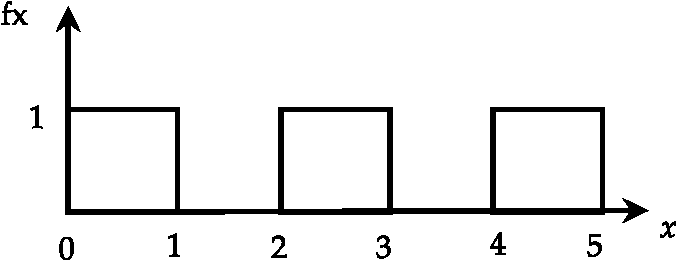
\includegraphics[height=2.5cm,width=6cm]{LT-01}
	\end{figure}
	Its Laplace transform $\tilde{f}(\mathrm{s})$ is
	 \begin{tasks}(2)
		\task[\textbf{a.}]$\frac{1+e^{-s}}{s}$
		\task[\textbf{b.}]$\frac{1-e^{-s}}{s}$
		\task[\textbf{c.}]$\frac{1}{s\left(1+e^{-s}\right)}$
		\task[\textbf{d.}]  $\frac{1}{s\left(1-e^{-s}\right)}$
	\end{tasks}
\end{exercise}
\begin{answer}
	Given function is a periodic function of period $T=2$
	\begin{align*}
	L[f(x)] &=\frac{1}{1-e^{-s T}} \int_{0}^{T} e^{-s x} f(x) d x=\frac{1}{1-e^{-2 s}} \int_{0}^{2} e^{-s x} d x \\
	&=\frac{1}{1-e^{-2 s}}\left[\int_{0}^{1} e^{-s x} d x\right]=\frac{1}{1-e^{-2 s}}\left(\frac{1-e^{-s}}{s}\right) \\
	&=\frac{\left(1-e^{-s}\right)}{s\left(1+e^{-s}\right)\left(1-e^{-s}\right)}=\frac{1}{s\left(1+e^{-s}\right)}
	\end{align*}
	So the correct answer is \textbf{option (c)}
\end{answer}
\begin{exercise}
	The inverse transform of $\frac{1}{s^2(s+1)}$ is
	 \begin{tasks}(2)
		\task[\textbf{a.}]$\frac{1}{2} t^{2} e^{-t}$
		\task[\textbf{b.}]$\frac{1}{2} t^{2}+1-e^{-t}$
		\task[\textbf{c.}]$t-1+e^{-t}$
		\task[\textbf{d.}] $\frac{1}{2} t^{2}\left(1-e^{-t}\right)$ 
	\end{tasks}
\end{exercise}
\begin{answer}
	\begin{align*}
	&f(s)=\frac{1}{s^{2}(s+1)}=\frac{(s+1)-s(s+1)+s^{2}}{s^{2}(s+1)}=\frac{1}{s^{2}}-\frac{1}{s}+\frac{1}{s+1} \\
	&\Rightarrow L^{-1}[f(s)]=t-1+e^{-t}
	\end{align*}
		So the correct answer is \textbf{option (c)}
\end{answer}

%\chapter{Fourier Transform }
\section{Integral Transforms}
Frequently in mathematical physics we encounter pairs of functions related by an expression of the form
\begin{equation}
g(x)=\int_{a}^{b} f(t) K(x, t) d t\label{FT-01}
\end{equation}
where it is understood that $a, b$, and $K(x, t)$ (called the kernel) will be the same for all function pairs $f$ and $g$. We can write the relationship expressed in Eq. (\ref{FT-01}) in the more symbolic form
\begin{equation}
g(x)=\mathcal{L} f(t)
\end{equation}
thereby emphasizing the fact that Eq. $(\ref{FT-01})$ can be interpreted as an operator equation. The function $g(x)$ is called the integral transform of $f(t)$ by the operator $\mathcal{L}$, with the specific transform determined by the choice of $a, b$, and $K(x, t)$. The operator defined by Eq. (\ref{FT-01}) will be linear:
\begin{align}
\int_{a}^{b}\left[f_{1}(t)+f_{2}(t)\right] K(x, t) d t&=\int_{a}^{b} f_{1}(t) K(x, t) d t+\int_{a}^{b} f_{2}(t) K(t) d t \\
\int_{a}^{b} c f(t) K(\alpha, t) d t&=c \int_{a}^{b} f(t) K(\alpha, t) d t
\end{align}
In order for transforms to be useful, we will shortly see that we need to be able to "undo" their effect. From a practical viewpoint, this means that not only must there exist an operator $\mathcal{L}^{-1}$, but also that we have a reasonably convenient and powerful method of evaluating
\begin{equation}
\mathcal{L}^{-1} g(x)=f(t)
\end{equation}
for an acceptably broad range of $g(x)$. The procedure for inverting a transform takes a wide variety of forms that depend on the specific properties of $K(x, t)$, so we cannot write a formula that is as general as that for $\mathcal{L}$ in Eq. (\ref{FT-01}).\\
Not all superficially reasonable choices for the kernel $K(x, t)$ will lead to operators $\mathcal{L}$ that have inverses, and even for strategically chosen kernels it may be the case that $\mathcal{L}$ and $\mathcal{L}^{-1}$ will only exist for substantially restricted classes of functions. Thus, the entire development of the present chapter is restricted (for any given integral transform) to functions for which the indicated operations can be carried out.\\
One of the frequent uses of integral transforms is to use one, together with its inverse, to form an \textbf{integral representation} of a function that we originally had in an explicit form. This move (which appears to be in the direction of generating greater complexity) has value that arises from the relatively simple behavior of the transforms of differentiation and integration operators. Procedures involving integral representations are also presented in later sections of this chapter.
\begin{figure}[H]
	\centering
	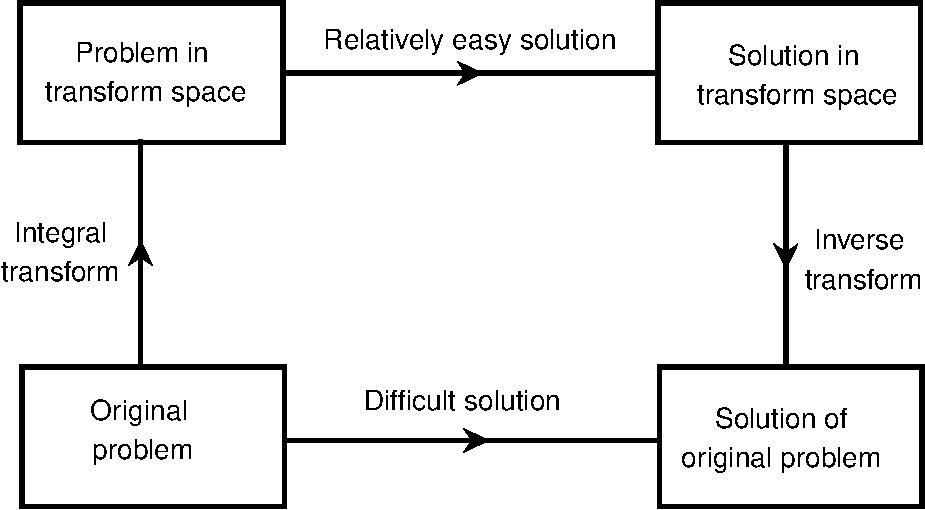
\includegraphics[height=5cm,width=9cm]{FT-01}
\end{figure}
\section{Some Important Transforms}
The integral transform that has seen the widest use is the Fourier transform, defined as
\begin{equation}
g(\omega)=\frac{1}{\sqrt{2 \pi}} \int_{-\infty}^{\infty} f(t) e^{i \omega t} d t
\end{equation}
The notation for this transform is not entirely universal; some writers omit the prefactor $1 / \sqrt{2 \pi}$; we keep it because it causes the transform and its inverse to have formulas that are more symmetrical. In applications involving periodic systems, one occasionally encounters a definition with kernel $\exp \left(2 \pi i \omega t / a_{0}\right)$, where $a_{0}$ is a lattice constant. These differences in notation do not change the mathematics, but cause formulas to differ by powers of $2 \pi$ or $a_{0}$. Caution is therefore advised when combining material from different sources.\\
\section{Infinite Fourier Transform}
\begin{align*}
\text{The fourier transform of }f(x)[-\infty<x<\infty] &:\\
f(s)=F\{f(x)\}&=\frac{1}{\sqrt{2 \pi}} \int_{-\infty}^{\infty} f(x) e^{i s x} d x\\
\text{Inverse fourier transform of }f(s)[-\infty<x<\infty] &:\\
f(x)=F^{-1}\{f(s)\}&=\frac{1}{\sqrt{2 \pi}} \int_{-\infty}^{\infty} f(s) e^{-i s x} d s .
\end{align*}
\section{Fourier Sine Transform}
\begin{align*}
f_{s}(\mathrm{~s})&=F_{s}\{f(x)\}=\sqrt{\frac{2}{\pi}} \int_{0}^{\infty} f(x) \sin s x d x \\
f(x)&=F_{s}^{-1}\left\{f_{s}(s)\right\}=\sqrt{\frac{2}{\pi}} \int_{0}^{\infty} f_{s}(s) \sin s x d s
\end{align*}
\section{Fourier Cosine Transform}
\begin{align*}
f_{c}(s)&=F_{c}\{f(x)\}=\sqrt{\frac{2}{\pi}} \int_{0}^{\infty} f(x) \cos s x d x \\
f(x)&=F_{c}^{-1}\left\{f_{c}(s)\right\}=\sqrt{\frac{2}{\pi}} \int_{0}^{\infty} f_{c}(s) \cos s x d s
\end{align*}
\subsubsection{Important Formulas:}
\begin{enumerate}
	\item $\int_{0}^{\infty} \frac{\sin a x}{x} d x=\frac{\pi}{2}$
	\item $\int_{0}^{\infty} e^{-x^{2}} d x=\sqrt{\frac{\pi}{2}}$
	\item $\int_{0}^{\infty} e^{-a x} \sin b x d x=\frac{b}{a^{2}+b^{2}}$
	\item $\int_{0}^{\infty} e^{-a x} \cos b x d x=\frac{a}{a^{2}+b^{2}}$
	\item $\int_{0}^{\infty} e^{-a x^{2}} d x=\frac{1}{2} \sqrt{\frac{\pi}{a}}$
	\item $\int_{0}^{\infty} e^{-a x^{2}} \cos b x d x=\frac{1}{2} \sqrt{\frac{\pi}{a}} e^{-b^{2} / 4 a}$
	\item $\int_{-\infty}^{\infty} e^{-a x^{2}+b x} d x=\sqrt{\frac{\pi}{a}} e^{b^{2} / 4 a}$
\end{enumerate}

\begin{exercise}
	Find the fourier transform of Gaussian distribution function $f(x)=N e^{-a x^{2}}$ where $N$ and 'a' are constant.
\end{exercise}
\begin{answer}
	\begin{align*}
	F\{f(x)\}=\frac{1}{\sqrt{2 \pi}} \int_{-\infty}^{\infty} f(x) e^{i k x} d x=\frac{1}{\sqrt{2 \pi}} \int_{-\infty} N e^{-a x^{2}} e^{i k x} d x=\frac{N}{\sqrt{2 \pi}} e^{-k^{2} / 4 a}
	\end{align*}
\end{answer}
\begin{exercise}
	Find $F\{\delta(x)\}$
\end{exercise}
\begin{answer}
	\begin{align*}
	F\{f(x)\}=\frac{1}{\sqrt{2 \pi}} \int_{-\infty}^{\infty} f(x) e^{i k x} d x=\frac{1}{\sqrt{2 \pi}} \int_{-\infty}^{\infty} \delta(x) e^{i k x} d x=\frac{1}{\sqrt{2 \pi}}\left[\mathrm{e}^{i k x}\right]_{x=0}=\frac{1}{\sqrt{2 \pi}}
	\end{align*}
\end{answer}
\begin{exercise}
	Find the fourier transform of $f(x)=e^{-a|x|} \quad(-\infty<x<\infty) \quad(a>0)$
\end{exercise}
\begin{answer}
	\begin{align*}
	\begin{aligned}
	F\left[e^{-a|x|}\right] &=\frac{1}{\sqrt{2 \pi}}\left[\int_{-\infty}^{0} e^{a x} e^{i s x} d x+\int_{0}^{\infty} e^{-a x} e^{i s x} d x\right]=\frac{1}{\sqrt{2 \pi}}\left[\left(\frac{e^{(a+i s) x}}{(a+i s)}\right)_{-\infty}^{0}+\left(\frac{e^{-(a-i s) x}}{(i s-a)}\right)_{0}^{\infty}\right] \\
	&=\frac{1}{\sqrt{2 \pi}}\left[\frac{1}{a+i s}+\frac{1}{a-i s}\right]=\frac{2 a}{\sqrt{2 \pi}\left(s^{2}+a^{2}\right)} \because
	\end{aligned}
	\end{align*}
\end{answer}

\section{Properties of Fourier Transform}
(i) \textbf{Linearity theorem:} 
\begin{align*}
\text{If }F(x)&=a_{1} f_{1}(x)+a_{2} f_{2}(x)+\ldots\text{ then, }\\f(s)&=F[f(x)]=a_{1} f_{1}(s)+a_{2} f_{2}(s)+\ldots
\end{align*}
(ii) \textbf{Change of scale property: }
\begin{align*}
\text{If }F[f(x)]&=f(s),\text{ then }F\{f(a x)\}\\&=\frac{1}{a} f(\mathrm{~s} / a)
\end{align*}
(iii) $\text{If }F\{f(x)\}=f(s),\text{ then }F\left\{f^{*}(x)\right\}=f^{*}(-s)$\\\\
(iv) \textbf{Shifting property:}
 \begin{align*}
\text{ If $f(s)$ is the Fourier transform of }\mathrm{f}(\mathrm{x}), \text{ then }F\{f(x \pm a)\}=e^{\mp i s a} f(s)
 \end{align*}
(v) \textbf{Modulation theorem:} \\\\
If $F\{f(x)\}=f(s)$, then $F\{f(x) \cos a x\}=\frac{1}{2} f(s-a)+\frac{1}{2} f(s+a)$
\section{Parseval Identity for Fourier Transform}
If the Fourier transform of $f(x)$ and $g(x)$ be $f(s) \& g(s)$ respectively, then\\\\
(i) $\int_{-\infty}^{\infty} f(s) g^{*}(s) d s=\int_{-\infty}^{\infty} f(x) g^{*}(x) d x$\\\\
where $g^{*}(s)$ is complex conjugate of $g(s)$ and $g^{*}(x)$ is the complex conjugate of $g(x)$.\\\\
(ii) $\left.\int_{-\infty}^{\infty}|f(s)|\right.^{2} d s=\int_{-\infty}^{\infty}|f(x)|^{2} d x$
\begin{exercise}Using parseval's identity show that $\int_{b}^{\infty}\left(\frac{\sin x}{x}\right)^{2} d x=\pi / 2$
\end{exercise}
\begin{answer}
	\begin{align*}
	F\{f(x)\}&=\frac{1}{\sqrt{2 \pi}} \int_{-\infty}^{\infty} f(x) e^{i x x} d x=\sqrt{\frac{2}{\pi}} \frac{\sin a s}{s}\\
	\text{Using parseval identity, }\int_{-\infty}^{\infty}|f(x)|^{2} d x&=\int_{-\infty}^{\infty}|f(s)|^{2} d s\\
	\int_{-a}^{\infty} l^{2} d x&=\int_{-\infty}^{\infty} \frac{2}{\pi} \frac{\sin ^{2} a s}{s^{2}} d s \\ 2 a&=\frac{2}{\pi} \int_{-\infty}^{\infty}\left(\frac{\sin a s}{s}\right)^{2} d s\\
	\text{Putting }a s&=x \Rightarrow a d s=d x\\
	\Rightarrow \pi&=\int_{-\infty}^{\infty}\left(\frac{\sin x}{x}\right)^{2} d x \\ \int_{0}^{\infty}\left(\frac{\sin x}{x}\right)^{2} d x&=\frac{\pi}{2}
	\end{align*}
\end{answer}
\begin{exercise}
	If the fourier transform of $f(x)$ is $f(s)$, then find the fourier transform of $\frac{d f}{d x}$
\end{exercise}
\begin{answer}
	\begin{align*}
	F\left[\frac{d f}{d x}\right]&=\frac{1}{\sqrt{2 \pi}} \int_{-\infty}^{\infty} \frac{d f}{d x} e^{i s x} d x\\&=\frac{1}{\sqrt{2 \pi}}\left[e^{i s x} f(x)\right]_{-\infty}^{\infty}-\frac{1}{\sqrt{2 \pi}} \int_{-\infty}^{\infty} i s e^{i s x} f(x) d x\\
	\intertext{Since $f(x)$ should be a well behave function for the fourier tranform to exist, therefore, the first term of the above equation should be equal to zero.}
	\text{Then }F\left[\frac{d f}{d x}\right]&=-i s \frac{1}{\sqrt{2 \pi}} \int_{-\infty}^{\infty} e^{i s x} f(x) d x=-is f( {s})
	\end{align*}
\end{answer}
\begin{exercise}
	Find Fourier transform of $f(x)= \begin{cases}x^{2}, & |x|<a \\ 0, & |x|>a\end{cases}$
\end{exercise}
\begin{answer}
	\begin{align*}
	F\{f(x)\} &=\frac{1}{\sqrt{2 \pi}} \int_{-\infty}^{\infty} e^{i s x} f(x) d x=\frac{1}{\sqrt{2 \pi}} \int_{-a}^{a} e^{i s x} x^{2} d x \\
	&=\frac{1}{\sqrt{2 \pi}}\left[\left(\frac{e^{i s x}}{i s} \cdot x^{2}\right)_{x=-a}^{a}-\frac{2}{i s} \int_{-a}^{a} x e^{i s x} d x\right] \\
	&=\frac{1}{\sqrt{2 \pi}}\left[\frac{a^{2}}{i s}\left(e^{i s a}-e^{-i s a}\right)-\frac{2}{i s}\left[\left(\frac{x e^{i s x}}{i s}\right)_{x=-a}^{a}-\frac{1}{i s} \int_{-a}^{a} e^{i s x} d x\right]\right]\\
	&=\frac{1}{\sqrt{2 \pi}}\left[\frac{2 a^{2}}{s} \sin (s a)+\frac{2 a}{s^{2}} \cos (s a)-\frac{4}{s^{3}} \sin (s a)\right]
	\end{align*}
\end{answer}
\begin{exercise}
	Find the complex fourier transform $e^{-|x|}$
\end{exercise}
\begin{answer}
	\begin{align*}
	F\left\{e^{-|x|}\right\}&=\frac{1}{\sqrt{2 \pi}} \int_{-\infty}^{\infty} e^{-|x|} e^{i s x} d x\\&=\frac{1}{\sqrt{2 \pi}}\left[\int_{-\infty}^{0} e^{-|x|} e^{i s x} d x+\int_{0}^{\infty} e^{-|x|} \cdot e^{i s x} d x\right]\\
	&=\frac{1}{\sqrt{2 \pi}}\left[\int_{-\infty}^{0} e^{x} \cdot e^{i s x} d x+\int_{0}^{\infty} e^{-x(1-i s)} d x\right]\\&=\frac{1}{\sqrt{2 \pi}}\left[\left[\frac{e^{x(1+i s)}}{1+i s}\right]_{x=-\infty}^{0}+\left[\frac{e^{-x(1-i s)}}{-(1-i s)}\right]_{x=0}^{\infty}\right] \\
	&=\frac{1}{\sqrt{2 \pi}}\left[\frac{1}{1-i s}+\frac{1}{1+i s}\right]\\&=\frac{1}{\sqrt{2 \pi}}\left(\frac{2}{1+s^{2}}\right)
	\end{align*}
\end{answer}


\begin{exercise}
	The graph of a real periodic function $f(x)$ for the range $[-\infty, \infty]$ is shown below
	\begin{figure}[H]
		\centering
		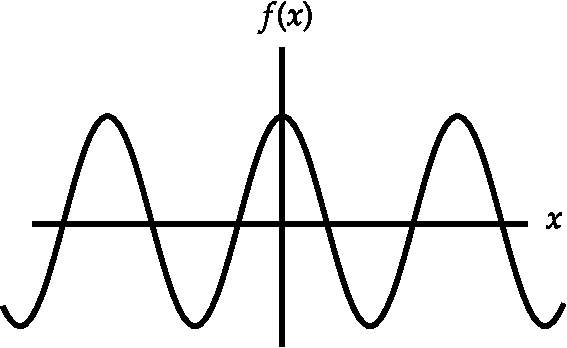
\includegraphics[height=3cm,width=5cm]{FT01}
	\end{figure}
	Which of the following graphs represents the real part of its Fourier transform?
	 \begin{tasks}(2)
		\task[\textbf{a.}]
		\begin{figure}[H]
			\centering
			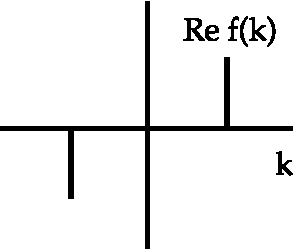
\includegraphics[height=2cm,width=2.5cm]{FT-06}
		\end{figure}
		\task[\textbf{b.}]	\begin{figure}[H]
			\centering
			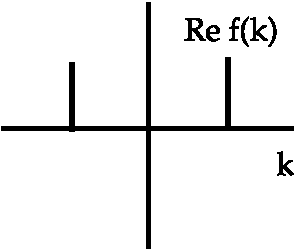
\includegraphics[height=2cm,width=2.5cm]{FT-05}
		\end{figure}
		\task[\textbf{c.}]	\begin{figure}[H]
			\centering
			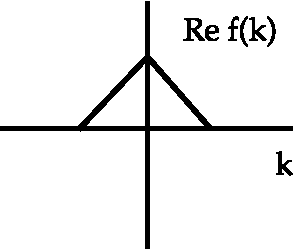
\includegraphics[height=2cm,width=2.5cm]{FT-03}
		\end{figure}
		\task[\textbf{d.}] 	\begin{figure}[H]
			\centering
			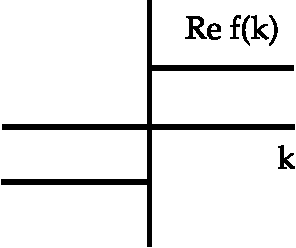
\includegraphics[height=2cm,width=2.5cm]{FT02}
		\end{figure}
	\end{tasks}
\end{exercise}
\begin{answer}
	\begin{align*}
	\text { The given graph in the question is of } f(x)&=\cos \omega x\\
	F(\cos \omega x)=\frac{1}{\sqrt{2 \pi}} \int_{-\infty}^{+\infty} \cos \omega x e^{i k x} d x&=\frac{1}{\sqrt{2 \pi}}\left(\int_{-\infty}^{+\infty} \frac{e^{i(k+\omega) x}}{2} d x+\int_{-\infty}^{+\infty} \frac{e^{i(k-\omega) x}}{2} d x\right)\\
	&\Rightarrow F(\cos \omega x) \frac{1}{\sqrt{2 \pi}}\left(\frac{1}{2} \delta(k+\omega)+\frac{1}{2} \delta(k-\omega)\right)
	\intertext{Therefore, the fourier transform of $f(x)=\cos x \omega x$ consist of two delta functions of same height at $k=\omega$ and $k=-\omega$.}
	\end{align*}
		So the correct answer is \textbf{option (b)}
\end{answer}
\newpage
\begin{abox}
	Practise Set-1
\end{abox}
\begin{enumerate}

\item The Fourier transform of the derivative of the Dirac $\delta-$ function, namely $\delta^{\prime}(x)$, is proportional to
{\exyear{NET/JRF(DEC-2013)}}

\begin{tasks}(4)
\task[\textbf{A.}] 0
\task[\textbf{B.}] 1
\task[\textbf{C.}] $\sin k$
\task[\textbf{D.}] $i k$
\end{tasks}
\item 
	The graph of a real periodic function $f(x)$ for the range $[-\infty, \infty]$ is shown below {\exyear{NET/JRF(DEC-2014)}}
	\begin{figure}[H]
		\centering
		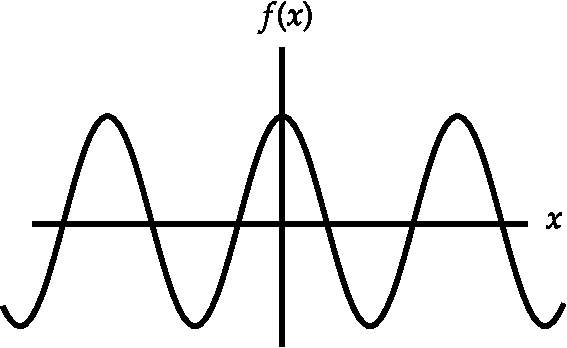
\includegraphics[height=3cm,width=5cm]{FT01}
	\end{figure}
	Which of the following graphs represents the real part of its Fourier transform?
	\begin{tasks}(2)
		\task[\textbf{A.}]
		\begin{figure}[H]
			\centering
			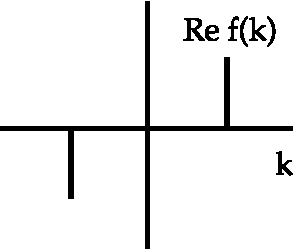
\includegraphics[height=2cm,width=2.5cm]{FT-06}
		\end{figure}
		\task[\textbf{B.}]	\begin{figure}[H]
			\centering
			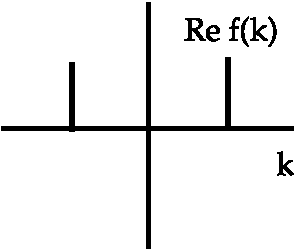
\includegraphics[height=2cm,width=2.5cm]{FT-05}
		\end{figure}
		\task[\textbf{C.}]	\begin{figure}[H]
			\centering
			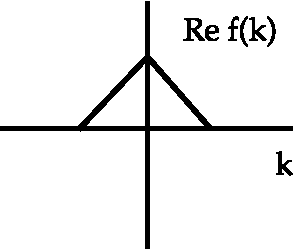
\includegraphics[height=2cm,width=2.5cm]{FT-03}
		\end{figure}
		\task[\textbf{D.}] 	\begin{figure}[H]
			\centering
			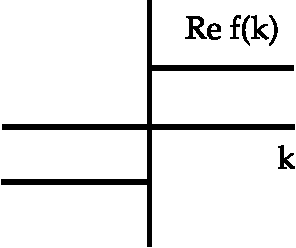
\includegraphics[height=2cm,width=2.5cm]{FT02}
		\end{figure}
	\end{tasks}
\item The Fourier transform of $f(x)$ is $\tilde{f}(k)=\int_{-\infty}^{+\infty} d x e^{i k x} f(x)$.
If $f(x)=\alpha \delta(x)+\beta \delta^{\prime}(x)+\gamma \delta^{\prime \prime}(x)$, where $\delta(x)$ is the Dirac delta-function (and prime denotes derivative), what is $\tilde{f}(k) ?$
{\exyear{NET/JRF(DEC-2015)}}

\begin{tasks}(2)
\task[\textbf{A.}] $\alpha+i \beta k+i \gamma k^{2}$
\task[\textbf{B.}] $\alpha+\beta k-\gamma k^{2}$
\task[\textbf{C.}]  $\alpha-i \beta k-\gamma k^{2}$
\task[\textbf{D.}] $i \alpha+\beta k-i \gamma k^{2}$
\end{tasks}
\item What is the Fourier transform $\int d x e^{i l x} f(x)$ of
$$
f(x)=\delta(x)+\sum_{n=1}^{\infty} \frac{d^{n}}{d x^{n}} \delta(x)
$$
where $\delta(x)$ is the Dirac delta-function?
{\exyear{NET/JRF(JUNE-2016)}}

\begin{tasks}(4)
\task[\textbf{A.}]  $\frac{1}{1-i k}$
\task[\textbf{B.}] $\frac{1}{1+i k}$
\task[\textbf{C.}] $\frac{1}{k+i}$
\task[\textbf{D.}] $\frac{1}{k-i}$
\end{tasks}
\item The Fourier transform $\int_{-\infty}^{\infty} d x f(x) e^{i k x}$ of the function $f(x)=\frac{1}{x^{2}+2}$ is
{\exyear{NET/JRF(DEC-2016)}}

\begin{tasks}(4)
\task[\textbf{A.}] $\sqrt{2} \pi e^{-\sqrt{2}|| \mid}$
\task[\textbf{B.}] $\sqrt{2} \pi e^{-\sqrt{2 k}}$
\task[\textbf{C.}] $\frac{\pi}{\sqrt{2}} e^{-\sqrt{2 k}}$
\task[\textbf{D.}] $\frac{\pi}{\sqrt{2}} e^{-\sqrt{2}|k|}$
\end{tasks}

\item The Fourier transform $\int_{-\infty}^{\infty} d x f(x) e^{i k x}$ of the function $f(x)=e^{-|x|}$
{\exyear{NET/JRF(JUNE-2018)}}

\begin{tasks}(4)
\task[\textbf{A.}] $-\frac{2}{1+k^{2}}$
\task[\textbf{B.}] $-\frac{1}{2\left(1+k^{2}\right)}$
\task[\textbf{C.}] $\frac{2}{1+k^{2}}$
\task[\textbf{D.}] $\frac{2}{\left(2+k^{2}\right)}$
\end{tasks}
\item The Heaviside function is defined as $H(t)=\left\{\begin{array}{ll}+1, & \text { for } t>0 \\ -1, & \text { for } t<0\end{array}\right.$ and its Fourier transform is given by $-2 i / \omega$. The Fourier transform of $\frac{1}{2}[H(t+1 / 2)-H(t-1 / 2)]$ is
{\exyear{GATE 2015}}

\begin{tasks}(4)
\task[\textbf{A.}] $\frac{\sin \left(\frac{\omega}{2}\right)}{\frac{\omega}{2}}$
\task[\textbf{B.}]  $\frac{\cos \left(\frac{\omega}{2}\right)}{\frac{\omega}{2}}$
\task[\textbf{C.}] $\sin \left(\frac{\omega}{2}\right)$
\task[\textbf{D.}]  0
\end{tasks}
\item The Fourier transform of the function $\frac{1}{x^{4}+3 x^{2}+2}$ up to proportionality constant is
{\exyear{JEST 2017}}

\begin{tasks}(2)
\task[\textbf{A.}] $\sqrt{2} \exp \left(-k^{2}\right)-\exp \left(-2 k^{2}\right)$
\task[\textbf{B.}]$\sqrt{2} \exp (-|k|)-\exp (-\sqrt{2}|k|)$
\task[\textbf{C.}] $\sqrt{2} \exp (-\sqrt{|k|})-\exp (-\sqrt{2|k|})$
\task[\textbf{D.}]$\sqrt{2} \exp \left(-\sqrt{2} k^{2}\right)-\exp \left(-2 k^{2}\right)$
\end{tasks}
\item The Laplace transform of $\frac{(\sin (a t)-a t \cos (a t))}{\left(2 a^{3}\right)}$ is 
{\exyear{JEST 2018}}

\begin{tasks}(4)
\task[\textbf{A.}] $\frac{2 a s}{\left(s^{2}+a^{2}\right)^{2}}$
\task[\textbf{B.}]$\frac{s^{2}-a^{2}}{\left(s^{2}+a^{2}\right)^{2}}$
\task[\textbf{C.}]$\frac{1}{(s+a)^{2}}$
\task[\textbf{D.}]$\frac{1}{\left(s^{2}+a^{2}\right)^{2}}$
\end{tasks}
\end{enumerate}
\colorlet{ocre1}{ocre!70!}
\colorlet{ocrel}{ocre!30!}
\setlength\arrayrulewidth{1pt}
\begin{table}[H]
	\centering
	\arrayrulecolor{ocre}
	\begin{tabular}{|p{1.5cm}|p{1.5cm}||p{1.5cm}|p{1.5cm}|}
		\hline
		\multicolumn{4}{|c|}{\textbf{Answer key}}\\\hline\hline
		\rowcolor{ocrel}Q.No.&Answer&Q.No.&Answer\\\hline
		1&\textbf{D} &2&\textbf{B}\\\hline 
		3&\textbf{C} &4&\textbf{B} \\\hline
		5&\textbf{D} &6&\textbf{C} \\\hline
		7&\textbf{A}&8&\textbf{B}\\\hline
		9&\textbf{D}&10&\textbf{}\\\hline
		11&\textbf{} &12&\textbf{}\\\hline
		13&\textbf{}&14&\textbf{}\\\hline
		15&\textbf{}& &\\\hline
		
	\end{tabular}
\end{table}
\newpage
\begin{abox}
	Practise Set-3
\end{abox}
\begin{enumerate}
	\item Let $F(k)$ is the Fourier exponential transform of $f(x)$ and $G(k)$ be the Fourier Transform of $g(x)=f(x+a)$. Then $G(k)$ is given by
	(Use the Fourier integral $F(k)=\frac{1}{\sqrt{2 \pi}} \int_{-\infty}^{+\infty} f(x) e^{i k x} d x$ )
	\begin{tasks}(2)
		\task[\textbf{a.}]$e^{i a k} f(k)$
		\task[\textbf{b.}]$e^{-i a k} F(-k)$
		\task[\textbf{c.}] $e^{-i a k} F(k)$
		\task[\textbf{d.}] $e^{-i a k} f(k)$
	\end{tasks}
	\begin{answer}
	\begin{align*}
	F(k)&=\frac{1}{\sqrt{2 \pi}} \int_{-\infty}^{+\infty} f(x) e^{i k x} d x\\
	\because g(x)&=f(x+a)\\
	\therefore G(k)&=\frac{1}{\sqrt{2 \pi}} \int_{-\infty}^{+\infty} f(x+a) e^{i k x} d x\\
	\text{Let }x+a&=y, d x=d y\\
	\therefore G(k)&=\frac{1}{\sqrt{2 \pi}} \int_{-\infty}^{+\infty} f(y) e^{i k(y-a)} d y=e^{-i k a} \frac{1}{\sqrt{2 \pi}} \int_{-\infty}^{+\infty} f(x) e^{i k x} d x=e^{-i a k} F(k)
	\end{align*}
	So the correct answer is \textbf{Option (c)}
\end{answer}
	\item The value of a function is given by $f(x)=\left\{\begin{array}{cc}1 & 0<x<1 \\ -1 & 1<x<2 \\ 0 & x>2\end{array}\right.$, the Fourier cosine transform of $f(x)$ is
	\begin{tasks}(2)
		\task[\textbf{a.}]$\sqrt{\frac{2}{\pi}}\left(\frac{2 \sin \omega+\sin 2 \omega}{\omega}\right)$
		\task[\textbf{b.}]$\sqrt{\frac{2}{\pi}}\left(\frac{2 \sin \omega-\sin 2 \omega}{\omega}\right)$
		\task[\textbf{c.}]$\sqrt{\frac{2}{\pi}}\left(\frac{\sin \omega-\sin 2 \omega}{\omega}\right)$
		\task[\textbf{d.}] $\sqrt{\frac{2}{\pi}}\left(\frac{2 \sin \omega}{\omega}\right)$
	\end{tasks}
\begin{answer}
	\begin{align*}
	f_{c}(\omega) &=\sqrt{\frac{2}{\pi}} \int_{0}^{\infty} f(x) \cos \omega x d x \\ &=\sqrt{\frac{2}{\pi}} \int_{0}^{1} \cos \omega x d x+\sqrt{\frac{2}{\pi}} \int_{1}^{2}-\cos \omega x d x \\ &=\sqrt{\frac{2}{\pi}}\left[\left(\frac{\sin \omega x}{\omega}\right)_{0}^{1}-\left(\frac{\sin \omega x}{\omega}\right)_{1}^{2}\right] \\ &=\sqrt{\frac{2}{\pi}}\left(\frac{2 \sin \omega-\sin 2 \omega}{\omega}\right) 
	\end{align*}
	So the correct answer is \textbf{Option (b)}
\end{answer}
	\item Consider the function $\delta_{n}(x)=\frac{n}{\sqrt{\pi}} \exp \left(-n^{2} x^{2}\right)$. For $n \rightarrow \infty$ The Fourier transform of the function is given by
	\begin{tasks}(2)
		\task[\textbf{a.}]$\delta(x)=\int_{-\infty}^{+\infty} e^{-i k x} d k$
		\task[\textbf{b.}]$\delta(x)=\frac{1}{2 \pi} \int_{-\infty}^{+\infty} e^{i k x} d k$
		\task[\textbf{c.}]$\delta(x)=\frac{1}{2 \pi} \int_{-\infty}^{+\infty} e^{-i k x} d k$
		\task[\textbf{d.}] 0
	\end{tasks}
	\begin{answer}
	\begin{align*}
	\mathrm{n}: g(k)&=\frac{1}{\sqrt{2 \pi}} \int_{-\infty}^{+\infty} \frac{n}{\sqrt{\pi}} e^{-n^{2} x^{2}} e^{i k x} d x=\frac{n}{\sqrt{2} \cdot \pi} \int_{-\infty}^{+\infty} e^{-n^{2} x^{2}+i i x} d x=\frac{n}{\sqrt{2} \cdot \pi} e^{-k^{2} / 4 n^{2}} \int_{-\infty}^{+\infty} e^{-n^{2}\left(x-\frac{i k}{2 n^{2}}\right)^{2}} d x\\
	&=\frac{n}{\sqrt{2} \cdot \pi} e^{-k^{2} / 4 n^{2}} \times 2 \times \frac{1}{2} \cdot \frac{\sqrt{\pi}}{n}=\frac{1}{\sqrt{2 \pi}} e^{-k^{2} / 4 n^{2}}
	\intertext{ Now inverse fourier transform of $g(k)$ is}
	\delta_{n}(x)&=\frac{1}{\sqrt{2 \pi}} \int_{-\infty}^{+\infty} \frac{e^{-k^{2} / 4 n^{2}}}{\sqrt{2 \pi}} \cdot e^{-i k x} d k\\
	\delta(x)&=\lim _{n \rightarrow \infty} \delta_{n}(x)=\lim _{n \rightarrow \infty} \frac{1}{2 \pi} \int_{-\infty}^{+\infty} e^{-k^{2} / 4 n^{2}} \cdot e^{-i k x} d k=\frac{1}{2 \pi} \int_{-\infty}^{+\infty} e^{-i k x} d k\\
	\therefore \delta(x)&=\frac{1}{2 \pi} \int_{-\infty}^{+\infty} e^{-i k x} d k
	\end{align*}
	So the correct answer is \textbf{Option (c)}
\end{answer}
	\item For the function $f(t)=\delta(t-x)$, the Fourier cosine integral is defined as $g_{c}(\omega)=\sqrt{\frac{2}{\pi}} \int_{0}^{\infty} f(t) \cos \omega t d t$. Its Fourier transform is:
	\begin{tasks}(2)
		\task[\textbf{a.}] $\sqrt{\frac{2}{\pi}} \cos \omega x$
		\task[\textbf{b.}]$\sqrt{\frac{2}{\pi}}$
		\task[\textbf{c.}]$\sqrt{\frac{2}{\pi}} \sin \omega x$
		\task[\textbf{d.}] $i \sqrt{\frac{2}{\pi}}$
	\end{tasks}
	\begin{answer}
	\begin{align*}
	\text{(i) }g_{c}(\omega)=\sqrt{\frac{2}{\pi}} \int_{0}^{\omega} \delta(t-x) \cos \omega t d t=\sqrt{\frac{2}{\pi}} \cos \omega x
	\end{align*}
	So the correct answer is \textbf{Option (a)}
\end{answer}
	\item $f(t)=\frac{\hbar}{2 \pi i} \int_{-\infty}^{+\infty} \frac{e^{-i \omega t} d \omega}{\left(E_{0}-i \Gamma / 2-\hbar \omega\right)}$ The value of $f(t)$ is given by
	\begin{tasks}(2)
		\task[\textbf{a.}](a) $f(t)= \begin{cases}e^{-\Gamma t / 2 \hbar} e^{-i E_{0} t / \hbar} & , t>0 \\ 0 & , t<0\end{cases}$
		\task[\textbf{b.}]$f(t)= \begin{cases}e^{\sqrt{1 / 2 \hbar}} e^{-1 E_{0} t / \hbar} & , t>0 \\ 0 & , t<0\end{cases}$
		\task[\textbf{c.}]$f(t)= \begin{cases}e^{-\Gamma t / 2 \hbar} e^{-i E_{0} t / \hbar} & , t>0 \\ 0 & , t<0\end{cases}$
		\task[\textbf{d.}] $f(t)= \begin{cases}e^{-\Gamma t / 2 h} e^{-i E_{0} t / h} & , t>0 \\ e^{-i E_{0} t / \hbar} & , t<0\end{cases}$
	\end{tasks}
	\begin{answer}
	\begin{align*}
	\intertext{Fourier Transform of $f(t)$ is}
	g(\omega)&=\frac{1}{\sqrt{2 \pi}} \int_{0}^{\infty} e^{-\Gamma t / 2 \hbar} \cdot e^{-i E_{0} / / \hbar} \cdot e^{i a t} d t=\frac{1}{\sqrt{2 \pi}} \int_{0}^{\infty} \exp \left\{\frac{-i t}{\hbar}\left(E_{0}-i \Gamma / 2-\hbar \omega\right)\right\} d t\\
	&=\frac{1}{\sqrt{2 \pi}}\left[\frac{e^{\left\{\frac{-i t}{\hbar}\left(E_{0}-i / / 2-\hbar \omega\right)\right\}}}{\frac{-i}{\hbar}\left(E_{0}-i \Gamma / 2-\hbar \omega\right)}\right]_{0}^{\infty}=\frac{1}{\sqrt{2 \pi}}\left[\frac{0-1}{\frac{-i}{\hbar}\left(E_{0}-i \Gamma / 2-\hbar \omega\right)}\right]\\
	&=\frac{1}{\sqrt{2 \pi} i(E o-i \Gamma / 2-h \omega)}
	\intertext{Inverse transform of $g(\omega)$ is}
	f(t)&=\frac{1}{2 \pi} \int_{-\infty}^{+\infty} \frac{\hbar e^{-i \omega x}}{i\left(E_{0}-i \Gamma / 2-\hbar \omega\right)} d \omega=\frac{\hbar}{2 \pi i} \int_{-\infty}^{+\infty} \frac{e^{-i \omega t} d \omega}{\left(E_{0}-i \Gamma / 2-\hbar \omega\right)}\\
	\therefore &\frac{\hbar}{2 \pi i} \int_{-\infty}^{+\infty} \frac{e^{-i \omega t} d \omega}{\left(E_{0}-i \Gamma / 2-\hbar \omega\right)}=f(t)= \begin{cases}\exp (-\Gamma t / 2 \hbar) \exp \left(\frac{-i E_{0} t}{\hbar}\right), & t>0 \\ 0 & t<0\end{cases}
	\end{align*}
	So the correct answer is \textbf{Option (c)}
\end{answer}
	\item The Fourier transform of function $h(t)=t e^{-t^{2}}$ is 
	\begin{tasks}(2)
		\task[\textbf{a.}] $j \pi f e^{-\pi^{2} f^{2}}$
		\task[\textbf{b.}]$-j \pi f e^{-\pi^{2} f^{2}}$
		\task[\textbf{c.}]$j \pi f e^{-\pi^{2} f^{2} / 4}$
		\task[\textbf{d.}] $-j \pi f e^{-\pi^{2} f^{2} / 4}$
	\end{tasks}
	\begin{answer}
	\begin{align*}
	F\left\{t e^{-r^{2}}\right\}&=-\frac{1}{2} F\left\{\frac{d\left(e^{-r^{2}}\right)}{d t}\right\}=-\frac{1}{2}(j 2 \pi f) F\left\{e^{-t^{2}}\right\}=-j \pi f e^{-\pi^{2} f^{2}}
	\end{align*}
	So the correct answer is \textbf{Option (b)}
\end{answer}
	\item The Fourier transform of the function $h(t)=\left\{\begin{array}{cc}\beta e^{-a t}, & t>0 \\ 0, & t<0\end{array}\right.$, is given by
	\begin{tasks}(2)
		\task[\textbf{a.}]$H(f)=\frac{\alpha}{\sqrt{\alpha^{2}+(2 \pi f)^{2}}} e^{j \tan ^{-1}\left[-2 \pi f^{\prime \alpha]}\right.}$
		\task[\textbf{b.}]$H(f)=\frac{\beta}{\sqrt{\alpha^{2}+(2 \pi f)^{2}}} e^{j \tan ^{-1}[-2 \pi f / \beta]}$
		\task[\textbf{c.}]$H(f)=\frac{\beta}{\sqrt{\alpha^{2}+(2 \pi f)^{2}}} e^{\tan ^{-1}[2 \pi f / \alpha]}$
		\task[\textbf{d.}] $H(f)=\frac{\beta}{\sqrt{\alpha^{2}+(2 \pi f)^{2}}} e^{j \tan ^{-1}[-2 \pi f / \alpha]}$
	\end{tasks}
	\begin{answer}
	\begin{align*}
	f(x)&=\left\{\begin{array}{rl}-1 & -1<x<0 \\ 1 & 0<x<1 \\ 0 & \text { otherwise }\end{array}\right.\\
	F[f(x)]&=\frac{1}{\sqrt{2 \pi}}\left[\int_{-1}^{0}-e^{-i \omega x} d x+\int_{0}^{1} e^{-i \omega x} d x\right]\\
	&=\frac{1}{\sqrt{2 \pi}}\left[-\left(\frac{e^{-i \omega x}}{-i \omega}\right)_{-1}^{0}+\left(\frac{e^{-i \omega x}}{-i \omega}\right)_{0}^{1}\right]=\frac{1}{\sqrt{2 \pi}}\left[\frac{-1+e^{i \omega}}{-i \omega}+\frac{e^{-i \omega}-1}{-i \omega}\right]\\
	&=\frac{1}{\sqrt{2 \pi}}\left[\frac{2 \cos \omega-2}{-i \omega}\right]=\frac{i}{\omega} \sqrt{\frac{2}{\pi}}(\cos \omega-1)
	\end{align*}
	So the correct answer is \textbf{Option (b)}
\end{answer}
	\item The Fourier transform of $f(x)=\left\{\begin{array}{cl}-1 & -1<x<0 \\ 1 & 0<x<1 \\ 0 & \text { otherwise }\end{array}\right.$ is
	\begin{tasks}(2)
		\task[\textbf{a.}] $\frac{i}{\omega} \sqrt{\frac{2}{\pi}}(\cos \omega+1)$
		\task[\textbf{b.}] $\frac{i}{\omega} \sqrt{\frac{2}{\pi}}(\cos \omega-1)$
		\task[\textbf{c.}]$-\frac{i}{\omega} \sqrt{\frac{2}{\pi}}(1+\cos \omega)$
		\task[\textbf{d.}] $\frac{i}{\omega} \sqrt{\frac{2}{\pi}}(1-\cos \omega)$
	\end{tasks}
	\begin{answer}
	\begin{align*}
	H(f)&=\int_{-\infty}^{+\infty} h(t) e^{-j 2 \pi f t} d t=\int_{0}^{+\infty} \beta e^{-\alpha t} e^{-j 2 \pi f t} d t=\beta \int_{0}^{+\infty} e^{-(\alpha+j 2 \pi f) t} d t\\
	\Rightarrow H(f)&=\left.\frac{-\beta}{\alpha+j 2 \pi f} e^{-(\alpha+j 2 \pi f) t}\right|_{0} ^{\infty}=\frac{\beta}{\alpha+j 2 \pi f}=\frac{\beta \alpha}{\alpha^{2}+(2 \pi f)^{2}}-j \frac{2 \pi f \beta}{\alpha^{2}+(2 \pi f)^{2}}\\
	\Rightarrow H(f)&=\frac{\beta}{\sqrt{\alpha^{2}+(2 \pi f)^{2}}} e^{j \tan ^{-1}[-2 \pi f / \alpha]}
	\end{align*}
	So the correct answer is \textbf{Option (d)}
\end{answer}
	\item The Fourier transform of $f(x)= \begin{cases}x, & 0<x<a \\ 0, & \text { otherwise }\end{cases}$ is
	\begin{tasks}(2)
		\task[\textbf{a.}]$\frac{1}{\sqrt{2 \pi} \cdot \omega^{2}}\left[e^{-i \omega n a}(1+i a \omega)-1\right]$
		\task[\textbf{b.}]$\frac{1}{\sqrt{2 \pi} \cdot \omega^{2}}\left[e^{-i \omega a}(1-i a \omega)-1\right]$
		\task[\textbf{c.}] $\frac{1}{\sqrt{2 \pi} \cdot \omega^{2}}\left[e^{-1 \text { tox }}(1+i a \omega)+1\right]$
		\task[\textbf{d.}] $\frac{1}{\sqrt{2 \pi} \cdot \omega^{2}}\left[e^{-i \omega a}(1-i a \omega)+1\right]$
	\end{tasks}
	\begin{answer}
	\begin{align*}
	f(x)&= \begin{cases}x, & 0<x<a \\ 0, & \text { otherwise }\end{cases}\\
	F[f(x)]&=\frac{1}{\sqrt{2 \pi}} \int_{0}^{a} x e^{-i \omega x} d x=\frac{1}{\sqrt{2 \pi}}\left[\left(\frac{x e^{-i e x}}{-i \omega}\right)_{0}^{a}-\left(\frac{e^{-i \omega x}}{(-i \omega)^{2}}\right)_{0}^{a}\right]\\&=\frac{1}{\sqrt{2 \pi}}\left[\frac{a e^{-i \omega a}}{-i \omega}-\frac{e^{-i \omega a}-1}{(-i \omega)^{2}}\right]=\frac{1}{\sqrt{2 \pi}}\left[\frac{i a \omega e^{-i e a}}{\omega^{2}}+\frac{e^{-i e a}-1}{\omega^{2}}\right]\\
	&=\frac{1}{\sqrt{2 \pi} \cdot \omega^{2}}\left[e^{-i \omega x}(1+i a \omega)-1\right]
	\end{align*}
	So the correct answer is \textbf{Option (a)}
\end{answer}


\item	If $F\left\{e^{-i 2 \text { avat }}\right\}=f(\omega+a)$, then $F(\cos 2 \pi v a t)=$ ?

\begin{answer}
	\begin{align*}
	\mathrm{F}[\cos 2 \pi v \mathrm{vat}]=\mathrm{F} \frac{\left[\mathrm{e}^{\mathrm{i} 2 \pi \mathrm{vat}}+\mathrm{e}^{-\mathrm{i} 2 \pi \mathrm{vat}}\right]}{2}=\frac{1}{2}\left\{F\left[e^{i 2 \pi v a t}\right]+F\left[e^{-i 2 \pi v a t}\right]\right\}=\frac{1}{2}[f(\omega-a)+f(\omega+a)]
	\end{align*}
\end{answer}

\item	Given that $F[\delta(x-a)]=\exp [-i 2 \pi v a]$, then $F^{-1}[\cos 2 \pi v a]=$ ?

\begin{answer}
	\begin{align*}
	\text{	As }\quad F\{\delta(x-a)\}&=\exp [-i 2 \pi v a] \quad \Rightarrow \delta(x-a)=F^{-1}[\exp (-i 2 \pi v a)]\\
	\text{Now }F^{-1}(\cos 2 \pi v a)&=F^{-1}\left[\frac{\exp (-i 2 \pi v a)+\exp (i 2 \pi v a)}{2}\right]=\frac{1}{2}[\delta(x+a)+\delta(x-a)]
	\end{align*}
\end{answer}

\item	Find the fourier cosine transform of the function $f(x)=e^{-a^{2} x^{2}}$

\begin{answer}
	\begin{align*}
	\begin{aligned}
	f_{c}(s) &=F_{c}[f(x)]=\sqrt{\frac{2}{\pi}} \int_{b}^{\infty} e^{-a^{2} x^{2}} \cos s x d x=\frac{1}{2} \sqrt{\frac{2}{\pi}} \int_{-\infty}^{\infty} e^{-a^{2} x^{2}} \cos s x d x \\
	&=\frac{1}{2} \sqrt{\frac{2}{\pi}} \text { Real part of } \int_{-\infty}^{\infty} e^{-a^{2} x^{2}} e^{i s x} d x=\frac{1}{2} \sqrt{\frac{2}{\pi}} \text { Real part of }\left(\sqrt{\frac{\pi}{a^{2}}} e^{\frac{i^{2} s^{2}}{4 a^{2}}}\right)=\frac{1}{\sqrt{2 a^{2}}} e^{-s^{2} / 4 a^{2}}
	\end{aligned}
	\end{align*}
\end{answer}

\item	Find the sine transform of $\frac{x}{1+x^{2}}$

\begin{answer}
	\begin{align}
	\text { Firstly we shall determine}&\text{ cosine transform of } \frac{1}{1+x^{2}}\notag\\
	F_{c}\left\{\frac{1}{1+x^{2}}\right\}&=\int_{0}^{\infty} \frac{\cos s x}{1+x^{2}} d x=I(\text { say })\notag\\
	\text{then }I&=\int_{0}^{\infty} \frac{\cos s x}{1+x^{2}} d x\label{FT-03}\\
	\text{Dufferentiating w.r.t.s,}\notag\\
	\frac{d I}{d s} &=\int_{0}^{\infty} \frac{-x \sin s x}{1+x^{2}} d x=F_{s}\left\{\frac{-x}{1+x^{2}}\right\}\label{FT-04} \\
	&=-\int_{0}^{\infty} \frac{x^{2} \sin s x d x}{x\left(1+x^{2}\right)}=-\int_{0}^{\infty} \frac{\left(1+x^{2}-1\right) \sin s x \cdot d x}{x\left(1+x^{2}\right)}\notag\\
	&=-\int_{0}^{\infty} \frac{\sin s x}{x} d x+\int_{0}^{\infty} \frac{\sin s x d x}{x\left(1+x^{2}\right)}=-\frac{\pi}{2}+\int_{0}^{\infty} \frac{\sin s x d x}{x\left(1+x^{2}\right)}\notag\\
	&=-\int_{0}^{\infty} \frac{\sin s x}{x} d x+\int_{0}^{\infty} \frac{\sin s x d x}{x\left(1+x^{2}\right)}=-\frac{\pi}{2}+\int_{0}^{\infty} \frac{\sin s x d x}{x\left(1+x^{2}\right)}\label{FT-05}\\
	\text{Differentiating again w.r.t. s,}\notag\\
	\frac{d^{2} I}{d s^{2}}&=\int_{0}^{\infty} \frac{x \cos (s x) d x}{x\left(1+x^{2}\right)}=I\notag\\
	\text { Or, } &\quad \frac{d^{2} I}{d s^{2}}-I=0\notag\\
	\text{The solution of it is }I&=A e^{-s}+B e^{s}\label{FT-06}\\
	\text{ Putting }\mathrm{s}&=0 \text{in (\ref{FT-03}),}\notag\\
	I &=\int_{0}^{\infty} \frac{1}{1+x^{2}} d x=\left(\tan ^{-1} x\right)_{0}^{\infty}=\frac{\pi}{2} \notag\\
	\therefore \quad I &=\frac{\pi}{2} \text { when } s=0\notag\\
	\text{Subjecting (\ref{FT-06}) to this}&\text{ condition}\notag\\
	\frac{\pi}{2}&=A+B\label{FT-07}
	\end{align}
\end{answer}
\item
	Find cosine transform of $f(x)$ if $f(x)= \begin{cases}\cos x, & 0<x<a \\ 0, & x>a\end{cases}$

\begin{answer}
	\begin{align*}
	F_{C}\{f(x)\} &=\sqrt{\frac{2}{\pi}} \int_{0}^{\infty} f(x) \cos (p x) d x \\
	&=\sqrt{\frac{2}{\pi}} \int_{0}^{a} \cos x \cos (p x) d x+\int_{a}^{\infty} 0 \cdot \cos p x d x \\
	&=\sqrt{\frac{2}{\pi}} \frac{1}{2} \int_{0}^{a}[\cos (p+1) x \cos (p-1) x] d x\\
	&=\sqrt{\frac{2}{\pi}} \frac{1}{2}\left[\frac{\sin (p+1) x}{p+1}+\frac{\sin (p-1) x}{p-1}\right]_{x=0}^{a} \\
	&=\sqrt{\frac{2}{\pi}} \frac{1}{2}\left[\frac{\sin (p+1) a}{p+1}+\frac{\sin (p-1) a}{p-1}\right]
	\end{align*}
\end{answer}

\item	Fourier transform of the derivative of the Dirac $\delta$-function, namely, $\delta^{\prime}(x)$, is proportional to
	\begin{tasks}(4)
		\task[\textbf{a.}]0
		\task[\textbf{b.}]1
		\task[\textbf{c.}] $\sin k$
		\task[\textbf{d.}] $\mathrm{i} k$
	\end{tasks}

\begin{answer}
	\begin{align*}
	\text { Fourier transform of } \delta^{\prime}(x)&=\frac{1}{\sqrt{2 \pi}} \int_{-\infty}^{\infty} \delta^{\prime}(x) e^{i k x} d x\\
	\intertext { Using the property of Dirac delta function, } \int_{-\infty}^{\infty} f(x) \delta^{\prime}(x-a) d x&=-f^{\prime}(a)\\
	\text { So, } \quad F\left[\delta^{\prime}(x)\right]&=-\frac{1}{\sqrt{2 \pi}}(i k)  \\ F\left[\delta^{\prime}(x)\right] &\propto i k
	\end{align*}
	So the correct answer is \textbf{option (d)}
\end{answer}
\end{enumerate}
%----------------------------------------------------------------------------------------
%	INDEX
%----------------------------------------------------------------------------------------

\cleardoublepage % Make sure the index starts on an odd (right side) page
\phantomsection
\setlength{\columnsep}{0.75cm} % Space between the 2 columns of the index
\addcontentsline{toc}{chapter}{\textcolor{ocre}{Index}} % Add an Index heading to the table of contents


%----------------------------------------------------------------------------------------

\end{document}
